\ifx\wholebook\relax \else
\documentclass[b5paper]{ctexart}
\usepackage[nomarginpar
  %, margin=.5in
]{geometry}

\addtolength{\oddsidemargin}{-0.05in}
\addtolength{\evensidemargin}{-0.05in}
\addtolength{\textwidth}{0.1in}
\usepackage[cn]{../../../prelude}

\setcounter{page}{1}

\begin{document}

\title{序列}

\author{刘新宇
\thanks{{\bfseries 刘新宇 } \newline
  Email: liuxinyu95@gmail.com \newline}
  }

\maketitle
\fi

\markboth{序列}{基本算法}

\ifx\wholebook\relax
\chapter{序列}
\numberwithin{Exercise}{chapter}
\fi

\section{简介}
\label{introduction}

序列是对数组和列表的一种抽象组合。我们希望理想的序列能达到下面的要求:

\begin{enumerate}
\item 可以在头部、尾部以常数时间插入、删除元素;
\item 可以快速(优于线性时间)连接两个序列;
\item 可以快速随机访问、更改任何元素;
\item 可以快速在指定位置断开序列。
\end{enumerate}

数组、列表仅部分满足这些要求,如下表所示。其中$n$为单个序列的长度,$n_1$、$n_2$分别表示被连接的两个序列的长度。

\btab{| l | c | r |}
  \hline
  操作 & 数组 & 列表 \\
  \hline
  在头部插入、删除 & $O(n)$ & $O(1)$ \\
  在尾部插入、删除 & $O(1)$ & $O(n)$ \\
  连接 & $O(n_2)$ & $O(n_1)$ \\
  随机访问 & $O(1)$ & 平均$O(n)$ \\
  在给定位置删除 & 平均$O(n)$ & $O(1)$ \\
  \hline
\etab

本章我们给出三种序列实现:二叉随机访问列表、可连接列表、手指树。

\section{二叉随机访问列表}
\index{序列!二叉随机访问列表}

二叉随机访问列表是由二叉树森林实现的随机访问列表。森林包含若干完全二叉树。元素只保存在叶子节点中。对任何非负整数$n$,将其表达为二进制,我们就知道需要多少棵完全二叉树来存储$n$个元素。每个值为1的二进制位代表一棵二叉树,树的大小对应着二进制位的高低。任给索引$1 \leq i \leq n$,我们都可以快速在森林中定位到保存第$i$个节点的二叉树。如图\ref{fig:bi-tree-sequence}所示,树$t_1$、$t_2$表示序列$[x_1, x_2, x_3, x_4, x_5, x_6]$。

\begin{figure}[htbp]
  \centering
  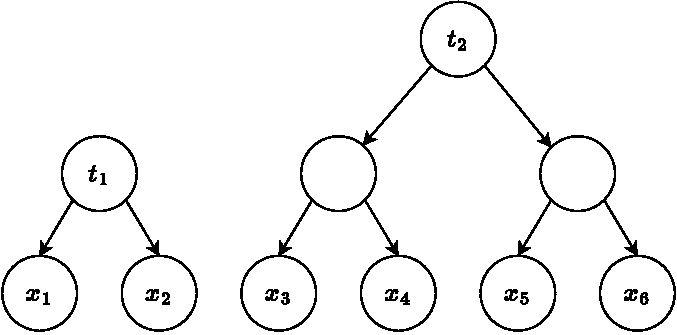
\includegraphics[scale=0.5]{img/bi-tree-sequence}
  \caption{含有6个元素的序列}
  \label{fig:bi-tree-sequence}
\end{figure}

记深度为$i+1$的完全二叉树为$t_i$。$t_0$只含有一个叶子节点。$t_i$含有$2^i$个叶子。对于$n$个元素的序列,我们把$n$表示为二进制数$n = (e_m e_{m-1} ... e_1 e_0)_2$,其中$e_i$为1或0。

\be
n = 2^0 e_0 + 2^1 e_1 + ... + 2^m e_m
\ee

如果$e_i \neq 0$,就需要一棵大小为$2^i$的完全二叉树$t_i$。在图\ref{fig:bi-tree-sequence}的例子中,序列长度为$6 = (110)_2$。最低位是0,我们不需要大小为1的树;第2位是1,需要一棵大小为2的树$t_1$;最高位是1,需要一棵大小为4的树$t_2$。这样就把序列$[x_1, x_2, ..., x_n]$表示为树的列表。列表中每棵树的大小都是唯一的,并按照从小到大排列。我们称之为\textbf{二叉随机访问列表}\cite{okasaki-book}。我们可以在二叉树定义的基础上稍作变化以实现这种列表:1、元素只保存在叶子节点中,2、在每棵子树中记录树的大小。这样每个分枝节点记为$(s, l, r)$,其中$s$表示子树的大小,$l$、$r$分别表示左右子树。包含元素$x$的叶子节点记为$(x)$。我们可以这样获取一棵树的大小:

\be
\begin{array}{rcl}
size\ (x) & = & 1 \\
size\ (s, l, r) & = & s \\
\end{array}
\ee

\index{二叉随机访问列表!插入}
为了把新元素$y$插入到序列$S$的前面,我们创建一棵只有一个叶子节点的$t_0$树:$t' = (y)$,然后把它插入到森林中。$insert\ y\ S = insert_T\ (y)\ S$,或写成克里化形式:

\be
insert\ y = insert_T\ (y)
\ee

我们检查森林中的第一棵树$t_i$,比较$t_i$和$t'$的大小,如果$t_i$较大,就将$t'$置于森林最前面(常数时间);若$t_i$和$t'$相等,我们将它们链接(常数时间)成一棵较大的树:$t'_{i+1} = (2s, t_i, t')$,然后递归地将$t'_{i+1}$插入到森林中。如图\ref{fig:bralist-2}所示。

\be
\begin{array}{rcl}
insert_T\ t\ [\ ] & = & [t] \\
insert_T\ t\ (t_1 \cons ts) & = & \begin{cases}
  size\ t < size\ t_1: & t : t_1 : ts \\
  \text{否则}: & insert_T\ (link\ t\ t_1)\ ts \\
  \end{cases}
\end{array}
\ee

其中$link$将两棵大小相同的树链接起来:$link\ t_1\ t_2 = (size\ t_1 + size\ t_2, t_1, t_2)$。

\begin{figure}[htbp]
  \centering
  \subcaptionbox{插入$x_1$。}{\hspace{0.2\textwidth}\includegraphics[scale=0.5]{img/bralst-1}\hspace{0.2\textwidth}}
  \subcaptionbox{插入$x_2$,链接产生$[t_1]$。}{\hspace{0.2\textwidth}\includegraphics[scale=0.5]{img/bralst-2}\hspace{0.2\textwidth}} \\
  \subcaptionbox{插入$x_3$,结果为$[t_0, t_1]$。}{\hspace{0.2\textwidth}\includegraphics[scale=0.5]{img/bralst-3}\hspace{0.2\textwidth}}
  \subcaptionbox{插入$x_4$。经两次链接后结果为$[t_2]$。}{\includegraphics[scale=0.5]{img/bralst-4}} \\
  \subcaptionbox{插入$x_5$,结果为:$[t_0, t_2]$。}{\includegraphics[scale=0.5]{img/bralst-5}}
  \subcaptionbox{插入$x_6$,结果为:$[t_1, t_2]$。}{\hspace{0.1\textwidth}\includegraphics[scale=0.5]{img/bralst-6}} \\
  \caption{插入$x_1, x_2, ..., x_6$}
  \label{fig:bralist-2}
\end{figure}

若森林中包含$m$棵树,$m$的大小为$O(\lg n)$,头部插入的性能为$O(\lg n)$。稍后我们证明分摊性能为$O(1)$。

\index{二叉随机访问列表!从头部删除}
对称地,我们利用插入的逆过程实现从序列头部删除元素。如果森林中第一棵树是$t_0$(单叶子节点),我们直接将$t_0$删除;否则,递归地将第一棵树拆分直到获得$t_0$,然后将其删除。如图\ref{fig:bralist-pop}所示。

\begin{figure}[htbp]
  \centering
  \subcaptionbox{序列$x_1, x_2, ..., x_5$对应森林$[t_0, t_2]$}{\includegraphics[scale=0.5]{img/bralst-5}}
  \subcaptionbox{删除$x_5$。直接删除$t_0$。}{\includegraphics[scale=0.5]{img/bralst-4}} \\
  \subcaptionbox{删除$x_4$。经过两次拆分后得到$[t_0, t_0, t_1]$,删除后得$[t_0, t_1]$。}{\hspace{0.2\textwidth}\includegraphics[scale=0.5]{img/bralst-3}\hspace{0.2\textwidth}}
  \caption{从头部删除元素}
  \label{fig:bralist-pop}
\end{figure}

\be
\begin{array}{rcl}
extract\ ((x) \cons ts) & = & (x, ts) \\
extract\ ((s, t_1, t_2) \cons ts) & = & extract\ (t_1 \cons t_2 \cons ts) \\
\end{array}
\ee

利用$extract$即可实现对头部元素的删除:

\be
\begin{cases}
head & = \textit{fst} \circ extract \\
tail & = \textit{snd} \circ extract \\
\end{cases}
\ee

其中$\textit{fst}\ (a, b) = a$, $\textit{snd}\ (a, b) = b$分别返回一对值中的两个部分。

\index{二叉随机访问列表!随机访问}
森林中的树实际上将元素划分为大小不同的区块。给定任意索引$1 \leq i \leq n$,我们先定位到对应的完全二叉树,然后再进行一次树查找就可定位到元素。

\begin{enumerate}
\item 比较$i$和森林中第一棵树$t$的大小,若$i \leq size(t)$,则元素在$t$中,接下来在树$t$中进行查找;
\item 否则,令$i' = i - size(t)$,然后递归地在剩余的树中查找第$i'$个元素。
\end{enumerate}

\be
(t \cons ts)[i] = \begin{cases}
  i \leq size\ t: & lookup_T\ i\ t \\
  \text{否则}: & ts[i - size\ t] \\
\end{cases}
\ee

其中$lookup_T$在树中进行二分查找。如果$i = 1$,我们返回根节点;否则,我们将树拆半,然后递归查找:

\be
\begin{array}{rcl}
lookup_T\ 1\ (x) & = & x \\
lookup_T\ i\ (s, t_1, t_2) & = & \begin{cases}
  i \leq \lfloor \dfrac{s}{2} \rfloor: & lookup_T\ i\ t_1 \\
  \text{否则}: & lookup_T\ (i - \lfloor \dfrac{s}{2} \rfloor)\ t_2 \\
  \end{cases}
\end{array}
\ee

图\ref{fig:get-at-example}描述了在一个长度为6的序列中查找第4个元素的步骤。第一棵树大小为2 < 4,继续检查第二棵树,并将索引更新为$i' = 4 - 2 $。接下来的树大小为$4 > i' = 2$,故待查找元素就在这棵树中。因为索引为2,不大于拆半的子树大小$4/2 = 2$,所以接下来检查左子树,然后检查右侧的孙子分支,最终得到要访问的元素。类似地,我们也可以修改任意位置$i$的元素。

\begin{figure}[htbp]
  \centering
  \subcaptionbox{$S[4], 4 > size(t_1) = 2$}{\includegraphics[scale=0.5]{img/bralst-6}}
  \subcaptionbox{$S'[4-2] \Rightarrow lookup_T\ 2\ t_2$}{\hspace{0.2\textwidth}\includegraphics[scale=0.5]{img/bralst-4}\hspace{0.2\textwidth}} \\
  \subcaptionbox{$ 2 \leq \lfloor \dfrac{size(t_2)}{2} \rfloor \Rightarrow lookup_T\ 2\ left(t_2)$}{\hspace{0.2\textwidth}\includegraphics[scale=0.5]{img/bralst-4l}\hspace{0.2\textwidth}}
  \subcaptionbox{$lookup_T\ 1\ right(left(t_2))$, 返回$x_3$}{\hspace{0.2\textwidth}\includegraphics[scale=0.5]{img/bralst-4lr}\hspace{0.2\textwidth}}
  \caption{获取$S[4]$}
  \label{fig:get-at-example}
\end{figure}

根据完全二叉树的性质,对于含有$n$个元素的序列,树木的棵数为$O(\lg n)$。对于索引$i$,最多需要$O(\lg n)$时间来定位到树。接下来的搜索和树的高度成正比,最多也是$O(\lg n)$。因此随机访问的总体性能为$O(\lg n)$。

\begin{Exercise}
如何处理索引越界情况?
\end{Exercise}

\section{数字表示}
\index{序列!二叉随机访问列表的数字表示}

在前一节,我们提到对于任意长度为$n$的序列,可以将$n$表示为二进制形式$n = 2^0e_0 + 2^1e_1 + ... + 2^me_m$,其中$e_i$为第$i$位,值为1或者0。若$e_i \neq 0$,则存在一棵大小为$2^i$的完全二叉树。

这一事实反映了$n$的二进制形式和森林之间存在明确的关系。向序列的头部插入元素,类似于将二进制数增加1;而从序列的头部删除元素类似于将二进制数减少1。我们称这种关系为\underline{numeric representation}\cite{okasaki-book}。

为了将二叉随机访问列表用二进制数字表示,可以为每一个二进制位定义两个状态。状态$Zero$表示不存在对应此二进制位大小的树,而$One$表示森林中存在一棵对应于此二进制位大小的树。如果状态为$One$,我们可以将对应的树附加到状态上。

下面的Haskell例子程序定义了这样状态。

\begin{lstlisting}[style=Haskell]
data Digit a = Zero
             | One (Tree a)

type RAList a = [Digit a]
\end{lstlisting}

我们重用了完全二叉树的定义,并把它附加到状态$One$上。同时将树的大小信息也加以缓存。

定义了数字(digit)后,一个森林就可以按照包含若干数字的列表来处理。我们首先看如何将新元素的插入操作实现为二进制数的增加。设函数$one(t)$创建一个$One$的状态,并将树$t$附加到这个状态上。函数$getTree(s)$从状态$s$中获取树。序列$S$是一个列表,包含若干表示状态的数字,记为$S = \{ s_1, s_2, ... \}$。$S'$为除第一个状态外的剩余部分。

\be
insertTree(S, t) = \left \{
  \begin{array}
  {r@{\quad:\quad}l}
  \{ one(t) \} & S = \phi \\
  \{ one(t) \} \cup S' & s_1 = Zero \\
  \{ Zero \} \cup insertTree(S', link(t, getTree(s_1))) & otherwise
  \end{array}
\right .
\ee

将一棵新树$t$插入到一个用二进制数字序列表示的森林$S$时,若森林为空,我们创建一个状态$One$,将待插入的树附加到状态上。这个状态是二进制数中的唯一一位。相当于二进制加法$0 + 1 = 1$。

否则,如果森林不为空,我们需要检查二进制数的第一位,如果第一个数字是$Zero$,我们创建一个状态$One$,附加上待插入的树,然后用这个新创建的$One$状态替换掉$Zero$状态。这相当于二进制加法$(...digits...0)_2 + 1 = (...digits...1)_2$。例如$6 + 1 = (110)_2 + 1 = (111)_2 = 7$。

最后一种情况是二进制数的第一位数字是$One$,这里我们假设待插入的树$t$和状态$One$中附加的树具有相同的size。这一点可以通过插入过程得到保证,我们总是从一个叶子开始插入,然后待插入的树的大小逐渐增长,呈一个序列$1, 2, 4, ..., 2^i, ...$。此时,我们将两棵树链接成一棵更大的树,然后递归地将链接结果插入到剩余的数字中。而之前的$One$状态,被替换为一个$Zero$状态。这相当于二进制加法$(...digits...1)_2 + 1 = (...digits'...0)_2$,其中$(...digits'...)_2 = (...digits...)_2+1$。例如$7 + 1 = (111)_2 + 1 = (1000)_2 = 8$。

下面的Haskell例子程序实现了这一算法。

\begin{lstlisting}[style=Haskell]
insertTree :: RAList a -> Tree a -> RAList a
insertTree [] t = [One t]
insertTree (Zero:ts) t = One t : ts
insertTree (One t' :ts) t = Zero : insertTree ts (link t t')
\end{lstlisting}

其他函数,包括$link()$、$cons()$等和此前的定义一样。

接下来我们解释如何用二进制数的减法来表示从序列的头部删除元素。如果序列只含有唯一的状态$One$,且状态上附加的树只有一个叶子。删除后序列变为空。这相当于二进制减法$1 - 1 = 0$。

否则,我们检查序列中的第一个数字,如果是$One$,它将被替换为$Zero$,表示森林中的这棵树将被删除。这相当于二进制减法 $(...digits...1)_2 - 1 = (...digits...0)_2$。例如$7 - 1 = (111)_2 - 1 = (110)_2 = 6$;

如果序列中的第一个数字是$Zero$,我们需要向后继的数字借位来进行删除。我们递归地从剩余的数字中抽取树,将其分拆成两棵子树。$Zero$状态将被替换成$One$状态,并将此前分拆出的右子树附加到状态上,而删除掉左子树。这相当于二进制减法$(...digits...0)_2 - 1 = (...digits'...1)_2$,其中$(...digits'...)_2 = (...digits...)_2 - 1$。例如$4 - 1 = (100)_2 - 1 = (11)_2 = 3$。下面的定义给出了删除算法。

\be
extractTree(S) = \left \{
  \begin{array}
  {r@{\quad:\quad}l}
  (t, \phi) & S = \{ one(t) \} \\
  (t, S') & s_1 = one(t) \\
  (t_l, \{ one(t_r) \} \cup S'' & otherwise
  \end{array}
\right .
\ee

其中$(t', S'') = extractTree(S')$,$t_l$和$t_r$分别是$t'$的左右子树。其他函数,包括$head$和$tail$的定义和此前一样。

使用数字表示二叉随机访问列表并没有改变复杂度,Okasaki在\cite{okasaki-ralist}中给出了详细地解释。作为例子,我们使用聚合(aggregation)法,来分析在头部插入的平均(或称分摊)复杂度。

考虑依次向一个空的二叉随机访问列表插入$n = 2^m$个元素的过程。森林的二进制表示可以列成表\ref{tab:ralist-insertion}:

\begin{table}[htbp]
\centering
\begin{tabular}{l | r}
  \hline
  i & 森林 (MSB ... LSB) \\
  \hline
  0 & 0, 0, ..., 0, 0 \\
  1 & 0, 0, ..., 0, 1 \\
  2 & 0, 0, ..., 1, 0 \\
  3 & 0, 0, ..., 1, 1 \\
  ... & ... \\
  $2^m-1$ & 1, 1, ..., 1, 1 \\
  $2^m$ & 1, 0, 0, ..., 0, 0 \\
  \hline
  位变化的次数 & 1, 1, 2, ... $2^{m-1}$, $2^m$ \\
  \hline
\end{tabular}
\caption{插入$2^m$个元素的过程中森林的二进制表示} \label{tab:ralist-insertion}
\end{table}

森林对应的LSB(最低位)每次在插入新元素时都变化,它总共需要$2^m$单位次计算;接下来的一位每隔一次变化,执行一次树的链接操作。总共需要$2^{m-1}$单位次计算;森林中对应MSB(最高位)的前一位总共只变化一次,它将此前所有的树链接成一棵更大的、森林中唯一的树,这发生在插入过程中的正中间。当最后一个元素插入后,MSB变化成1。

将所有的这些计算次数相加,我们得到$T = 1 + 1 + 2 + 4 + ... + 2^{m-1} + 2^m = 2^{m+1}$。因此平均下来每次插入操作的计算耗时:

\be
O(T/N) = O(\frac{2^{m+1}}{2^m}) = O(1)
\ee

这证明了插入算法的分摊复杂度为常数时间$O(1)$。删除算法复杂度的证明留给读者作为练习。

\subsection{命令式二叉随机访问列表}
\index{序列!命令式二叉随机访问列表}

使用二叉树实现命令式二叉随机访问列表非常简单,递归可以通过在循环中修改当前的树进行消除。我们将此作为练习留给读者。本节中,我们给出一些不同的命令式实现,但基本思路仍然是使用数值表示法。

回顾一下二叉堆一章中的内容。二叉堆可以通过隐式的数组来实现。我们可以借鉴类似的方法,用只含有一个元素的数组代表叶子;用含有2个元素的数组代表高度为1的二叉树;用含有$2^m$个元素的数组代表高度为$m$的完全二叉树。

这样做的好处是,我们可以通过索引快速访问任何元素,而无需进行分而治之的树查找。代价是树的链接操作被替换成了耗时的数组复制。

下面的ANSI C例子代码定义了二叉树森林。

\lstset{language=C}
\begin{lstlisting}
#define M sizeof(int) * 8
typedef int Key;

struct List {
    int n;
    Key* tree[M];
};
\end{lstlisting}

其中$n$是森林中存储的元素个数。当然,我们也可以通过使用动态数组来避免限制树的总数。例如下面的ISO C++例子程序。

\lstset{language=C++}
\begin{lstlisting}
template<typename Key>
struct List {
    int n;
    vector<vector<key> > tree;
};
\end{lstlisting}

简单起见,我们使用ANSI C作为例子。

首先回顾一下插入过程,若第一棵树为空(一个状态为$Zero$的数字),只需要将第一棵树变成一棵含有一个叶子节点的树,将待插入元素放入其中;否则,插入将引发树的链接,这一过程是递归的,直到某一个位置(digit),这个位置上对应的树为空。数值表示告诉我们,如果第一棵、第二棵、……、第$i-1$棵树都存在,而第$i$棵树为空,结果会构造一棵大小为$2^i$的树,待插入的元素,和所有此前的元素都存储在这棵树中。而位置$i$之后的所有树都保持不变。

怎样能高效地定位到位置$i$呢?如果使用二进制数来代表含有$n$个元素的森林,当插入一个新元素后,$n$增长到$n+1$。比较$n$和$n+1$的二进制形式可以发现,所有$i$之前的位都从1变到0,而第$i$位从0变成1,所有$i$之后的位都保持不变。我们可以用位运算异或($\oplus$)来检测到这一位,算法如下:

\begin{algorithmic}
\Function{Number-Of-Bits}{$n$}
  \State $i \gets 0$
  \While{$\lfloor \frac{n}{2} \rfloor \neq 0$}
    \State $ n \gets \lfloor \frac{n}{2} \rfloor$
    \State $ i \gets i + 1$
  \EndWhile
  \State \Return $i$
\EndFunction
\Statex
\State $i \gets $ \Call{Number-Of-Bits}{$n \oplus (n + 1)$}
\end{algorithmic}

也可以通过移位运算来计算一个二进制数中1的个数,如下面的ANSI C例子程序。

\begin{lstlisting}
int nbits(int n) {
    int i=0;
    while(n >>= 1)
      ++i;
    return i;
}
\end{lstlisting}

因此,命令式插入算法可以这样实现:首先定位到从0翻转成1的位$i$,然后创建一个大小为$2^i$的数组,用以代表相应的完全二叉树,最后将待插入元素和此位之前所有的内容移动到这一数组中。

\begin{algorithmic}
\Function{Insert}{$L, x$}
  \State $i \gets $ \Call{Number-Of-Bits}{$n \oplus (n + 1)$}
  \State \Call{Tree}{$L$}[$i+1$] $\gets $ \Call{Create-Array}{$2^i$}
  \State $l \gets 1$
  \State  \Call{Tree}{$L$}[$i+1$][$l$]  $\gets x$
  \For{$j \in [1, i]$}
    \For{$k \in [1, 2^j]$}
      \State $l \gets l + 1$
      \State \Call{Tree}{$L$}[$i+1$][$l$]  $\gets$ \Call{Tree}{$L$}[$j$][$k$]
    \EndFor
    \State \Call{Tree}{$L$}[$j$] $\gets$ NIL
  \EndFor
  \State \Call{Size}{$L$} $\gets$ \Call{Size}{$L$} + 1
  \State \Return $L$
\EndFunction
\end{algorithmic}

对应的ANSI C例子程序如下。

\lstset{language=C}
\begin{lstlisting}
struct List insert(struct List a, Key x) {
    int i, j, sz;
    Key* xs;
    i = nbits((a.n + 1) ^ a.n);
    xs = a.tree[i] = (Key*)malloc(sizeof(Key) * (1 << i));
    for(j = 0, *xs++ = x, sz = 1; j < i; ++j, sz << = 1) {
        memcpy((void*)xs, (void*)a.tree[j], sizeof(Key) * (sz));
        xs += sz;
        free(a.tree[j]);
        a.tree[j] = NULL;
    }
    ++a.n;
    return a;
}
\end{lstlisting}

但是这一方法的性能在理论上不如前面的好。这是因为原本常数时间的链接操作,下降成了线性时间的数组复制。

我们可以再次使用聚合法分析分摊性能。列表使用由数组表示的二叉树森林来实现,连续向一个空列表插入$n = 2^m$个元素,森林对应的二进制数变化和前面一样,但是每一个二进制位翻转时的计算量和此前有所不同,如表\ref{tab:imperative-ralist-insert}所示:

\begin{table}[htbp]
\centering
\begin{tabular}{l | r}
  \hline
  i & 森林 (MSB ... LSB) \\
  \hline
  0 & 0, 0, ..., 0, 0 \\
  1 & 0, 0, ..., 0, 1 \\
  2 & 0, 0, ..., 1, 0 \\
  3 & 0, 0, ..., 1, 1 \\
  ... & ... \\
  $2^m-1$ & 1, 1, ..., 1, 1 \\
  $2^m$ & 1, 0, 0, ..., 0, 0 \\
  \hline
  位变化的计算量 & $1 \times 2^m$, $1 \times 2^{m-1}$, $2 \times 2^{m-2}$, ... $2^{m-2} \times 2$, $2^{m-1} \times 1$ \\
  \hline
\end{tabular}
\caption{插入$2^m$个元素的过程中森林的二进制表示} \label{tab:imperative-ralist-insert}
\end{table}

森林的LSB每次插入新元素都会变化,但是只有在从0到1的变化时会创建含有一个叶子的树并进行复制,因此成本是$\frac{n}{2}$个计算单位,为$2^{m-1}$;下一位翻转的次数为LSB的一半,每当翻转成1时,就把待插入元素和第一棵树中的内容复制到第二棵树中。因此翻转一次的成本为2个计算单位,而不是1个;对于MSB,它在最后一次翻转成1,但是成本是将所有此前的树中的元素复制到大小为$2^m$的数组中。

将全部计算成本相加并除以插入次数$n$,就得到了分摊性能:

\be
\begin{array}{rcl}
O(T/N) & = & \displaystyle O(\frac{1 \times 2^m + 1 \times 2^{m-1} + 2 \times 2^{m-2} + ... + 2^{m-1} \times 1}{2^m}) \\
       & = & \displaystyle O(1 + \frac{m}{2}) \\
       & = & O(m)
\end{array}
\ee

因为$m = O(\lg n)$,所以分摊性能从常数时间下降为对数时间。但是这仍然比普通的数组插入要快,普通数组插入的平均性能为$O(n)$。

由于使用数组的索引,随机访问的性能要比此前的树查找更快。

\begin{algorithmic}
\Function{Get}{$L, i$}
  \For{each $t \in $ \Call{Trees}{$L$}}
    \If{$t \neq$ NIL}
      \If{$i \leq $ \Call{Size}{$t$}}
        \State \Return $t$[i]
      \Else
        \State $i \gets i -$ \Call{Size}{$t$}
      \EndIf
    \EndIf
  \EndFor
\EndFunction
\end{algorithmic}

简单起见,我们省略了索引越界的错误处理,相应的ANSI C例子程序如下:

\begin{lstlisting}
Key get(struct List a, int i) {
    int j, sz;
    for(j = 0, sz = 1; j < M; ++j, sz << = 1)
        if(a.tree[j]) {
            if(i < sz)
                break;
            i -= sz;
        }
    return a.tree[j][i];
}
\end{lstlisting}

命令式的删除和随机访问修改元素的算法留给读者作为练习。

\begin{Exercise}
\begin{enumerate}
\item 选择一门语言,实现数值表示的随机访问算法,包括查找和修改指定位置的元素。

\item 使用聚合法,证明删除算法的分摊复杂度为常数时间$O(1)$。

\item 选择一门命令式语言,设计并实现用数组表示的二叉随机访问列表。
\end{enumerate}
\end{Exercise}

\section{命令式双数组列表(paired-array list)}
\index{序列!双数组列表}

在前面的章节中,我们给出过一个用双数组(paired-array)实现的队列。在首尾两端都支持快速的操作。由于数组具备快速随机访问的性质,这一方法也可以用来实现命令式的列表。

\subsection{定义}
\index{双数组列表!定义}

图\ref{fig:palist}给出了双数组列表的结构。两个数组按照头对头的方式连接起来。在列表的头部插入元素时,新元素被添加到front数组的后尾;向列表的尾部插入元素时,新元素被添加到rear数组的末尾。

\begin{figure}[htbp]
  \centering
  \includegraphics[scale=1.0]{img/palist}
  \caption{一个双数组列表,包含两个头对头连接起来的数组} \label{fig:palist}
\end{figure}

下面的ISO C++例子程序定义了这样的一个数据结构。

\lstset{language=C++}
\begin{lstlisting}
template<typename Key>
struct List {
    int n, m;
    vector<Key> front;
    vector<Key> rear;

    List() : n(0), m(0) {}
    int size() { return n + m; }
};
\end{lstlisting}

这里我们使用了标准库提供的vector来简化动态内存管理。

\subsection{插入和添加}
\index{双数组列表!插入和添加}
令函数\textproc{Front}($L$)返回front数组,而\textproc{Rear}($L$)返回rear数组。简单起见,假设数组支持动态长度调整。插入和删除可以实现如下。

\begin{algorithmic}
\Function{Insert}{$L, x$}
  \State $F \gets $ \Call{Front}{$L$}
  \State \Call{Size}{$F$} $\gets $ \Call{Size}{$F$} + 1
  \State $F$[\Call{Size}{$F$}] $\gets x$
\EndFunction
\Statex
\Function{Append}{$L, x$}
  \State $R \gets $ \Call{Rear}{$L$}
  \State \Call{Size}{$R$} $\gets $ \Call{Size}{$R$} + 1
  \State $R$[\Call{Size}{$R$}] $\gets x$
\EndFunction
\end{algorithmic}

由于所有的操作都是在front数组和rear数组的末尾进行的,它们都是常数时间$O(1)$的。下面的ISO C++例子程序实现了这一算法。

\begin{lstlisting}
template<typename Key>
void insert(List<Key>& xs, Key x) {
    ++xs.n;
    xs.front.push_back(x);
}

template<typename Key>
void append(List<Key>& xs, Key x) {
    ++xs.m;
    xs.rear.push_back(x);
}
\end{lstlisting}

\subsection{随机访问}
\index{双数组列表!随机访问}
由于内部的数据结构是数组(动态数组vector),它支持随机访问,因此很容易实现索引算法。

\begin{algorithmic}
\Function{Get}{$L, i$}
  \State $F \gets $ \Call{Front}{$L$}
  \State $n \gets $ \Call{Size}{$F$}
  \If{$i \leq n $}
    \State \Return $F$[$n-i+1$]
  \Else
    \State \Return \Call{Rear}{$L$}[$i-n$]
  \EndIf
\EndFunction
\end{algorithmic}

这里索引$i \in [1, |L|]$。如果它不大于front数组的大小,则待访问的元素存储于front数组中。但因为front数组和rear数组是按照头对头的方式连接到一起的,所以front数组中的元素是按照“逆序”索引的。我们需要用数组的尺寸减去$i$来定位到元素;如果$i$大于front数组的大小,说明待访问的元素在rear数组中。而rear数组中的各个元素的顺序是正常的,我们只需要将$i$减去front数组的尺寸就可以定位到元素。

下面的ISO C++例子程序实现了这一算法。

\begin{lstlisting}
template<typename Key>
Key get(List<Key>& xs, int i) {
    if( i < xs.n )
        return xs.front[xs.n-i-1];
    else
        return xs.rear[i-xs.n];
}
\end{lstlisting}

随机访问修改元素的算法留给读者作为练习。

\subsection{删除和平衡}
\index{双数组列表!删除和平衡}
删除要比插入和添加复杂。这是因为删除可能造成一个数组(front数组或者rear数组)变空,而另外一个仍存有元素。极端情况下,列表会变得很不平衡。我们需要在这种情况下恢复平衡。

最简单的想法是当front或者rear数组变空时开始修复。我们可以将另外一个数组分成两半,然后将前一半反转顺序形成一对新的数组。算法描述如下:

\begin{algorithmic}
\Function{Balance}{$L$}
  \State $F \gets$ \Call{Front}{$L$}, $R \gets$ \Call{Rear}{$L$}
  \State $n \gets$ \Call{Size}{$F$}, $m \gets$ \Call{Size}{$R$}
  \If{ $F = \phi$}
    \State $F \gets$ \Call{Reverse}{$R$[1 ... $\lfloor \frac{m}{2} \rfloor$]}
    \State $R \gets R[\lfloor \frac{m}{2} \rfloor + 1$ ... $m]$
  \ElsIf{ $R = \phi$ }
    \State $R \gets$ \Call{Reverse}{$F$[1 ... $\lfloor \frac{n}{2} \rfloor$]}
    \State $F \gets F[\lfloor \frac{n}{2} \rfloor + 1$ ... $n]$
  \EndIf
\EndFunction
\end{algorithmic}

实际上front数组变空或rear数组变空引发的恢复平衡操作是对称的。我们可以交换front和rear数组,递归调用平衡恢复函数,最后在再把front和rear数组交换回来。下面的ISO C++例子程序实现了这一思路。

\begin{lstlisting}
template<typename Key>
void balance(List<Key>& xs) {
    if(xs.n == 0) {
        back_insert_iterator<vector<Key> > i(xs.front);
        reverse_copy(xs.rear.begin(), xs.rear.begin() + xs.m/2, i);
        xs.rear.erase(xs.rear.begin(), xs.rear.begin() +xs.m/2);
        xs.n = xs.m/2;
        xs.m -= xs.n;
    } else if(xs.m == 0) {
        swap(xs.front, xs.rear);
        swap(xs.n, xs.m);
        balance(xs);
        swap(xs.front, xs.rear);
        swap(xs.n, xs.m);
   }
}
\end{lstlisting}

定义好\textproc{Balance}算法后,就很容易实现头部和尾部的删除算法了。

\begin{algorithmic}
\Function{Remove-Head}{$L$}
  \State \Call{Balance}{$L$}
  \State $F \gets $ \Call{Front}{$L$}
  \If{$F = \phi$}
    \State \Call{Remove-Tail}{$L$}
  \Else
    \State \Call{Size}{$F$} $\gets $ \Call{Size}{$F$} - 1
  \EndIf
\EndFunction
\Statex
\Function{Remove-Tail}{$L$}
  \State \Call{Balance}{$L$}
  \State $R \gets $ \Call{Rear}{$L$}
  \If{$R = \phi$}
    \State \Call{Remove-Head}{$L$}
  \Else
    \State \Call{Size}{$R$} $\gets $ \Call{Size}{$R$} - 1
  \EndIf
\EndFunction
\end{algorithmic}

这里存在一种边界情况:恢复平衡后,待删除的数组仍然是空的。此时,使用双数组实现的列表中只有一个元素。我们只需要删除掉这唯一的元素,结果是一个空列表。下面的ISO C++程序实现了这一算法。

\begin{lstlisting}
template<typename Key>
void remove_head(List<Key>& xs) {
    balance(xs);
    if(xs.front.empty())
        remove_tail(xs); //删除rear中的唯一元素。
    else {
        xs.front.pop_back();
        --xs.n;
    }
}

template<typename Key>
void remove_tail(List<Key>& xs) {
    balance(xs);
    if(xs.rear.empty())
        remove_head(xs); //删除front中的唯一元素。
    else {
        xs.rear.pop_back();
        --xs.m;
    }
}
\end{lstlisting}

显然,最坏情况下性能为$O(n)$,其中$n$是双数组列表中存储的元素个数。最坏情况发生在平衡恢复被启动时,不论是逆序操作,还是shift操作都是线性时间的。但是删除算法的分摊复杂度仍然是$O(1)$,我们把证明作为练习留给读者。

\begin{Exercise}
\begin{enumerate}
\item 选择一门命令式语言实现随机访问的修改算法。
\item 我们使用了标准库中的vector来处理动态内存分配,请尝试用普通数组,自己管理内存分配来实现双数组列表,比较两个版本并分析算法的复杂度是否受到了影响。
\item 证明双数组列表删除算法的分摊复杂度为$O(1)$。
\end{enumerate}
\end{Exercise}

\section{可连接列表}
\index{序列!可链接列表}

通过使用二叉随机访问列表,我们实现了序列数据结构。支持在$O(\lg n)$时间的头部插入和删除,以及通过索引进行随机存取。

但是,将两个列表连接起来却并不容易。每个列表都是由完全二叉树组成的森林,我们不能简单地将它们合并到一起(森林本质上是树的列表,对于任何size,最多只存在一棵树的尺寸等于这一size。而且直接合并两个列表也并不快)。一个方法是将第一个序列中的元素逐一推入一个栈中,然后依次将栈中元素弹出并使用\texttt{cons}函数插入到第二个序列中。当然,栈可以通过使用递归来隐式实现,例如:

\be
concat(s_1, s_2) = \left \{
  \begin{array}
  {r@{\quad:\quad}l}
  s_2 & s_1 = \phi \\
  cons(head(s_1), concat(tail(s_1), s_2)) & otherwise
  \end{array}
\right .
\ee

其中函数$cons$、$head$和$tail$的定义和此前的一致。

如果两个序列的长度分别是$m$和$n$,这一方法首先用$O(n \lg n)$时间将第一个序列中的元素推入栈中,然后使用$\Omega(n \lg (n + m))$的时间将元素逐一插入的第二个序列的前面。其中$\Omega$表示上限,具体的定义可以参考\cite{CLRS}。

在前面章节中,我们实现了实时队列。他支持常数时间$O(1)$的入队和出队。如果我们能够将队列的连接操作实现为某种形式的入队操作,就可以将性能提高到常数时间。Okasaki在\cite{okasaki-book}中给出了这样的实现。

为了实现可连接列表,Okasaki设计了一种K叉树结构。树的根节点保存列表中的第一个元素,我们可以用常数时间$O(1)$访问到它。所有子树都是更小的可连接列表,保存在一个实时队列中。将另外一个列表连接到尾部相当于把这个列表添加为最后一个子树,这实际上是一个入队操作。添加新元素可以这样实现:首先将元素放入到一棵只有一个叶子节点的树中。然后将这棵树连接到序列的尾部从而完成添加。

图\ref{fig:clist}描述了这一数据结构。

\begin{figure}[htbp]
  \centering
  \subcaptionbox{列表$\{ x_1, x_2, ..., x_n\}$的数据结构}{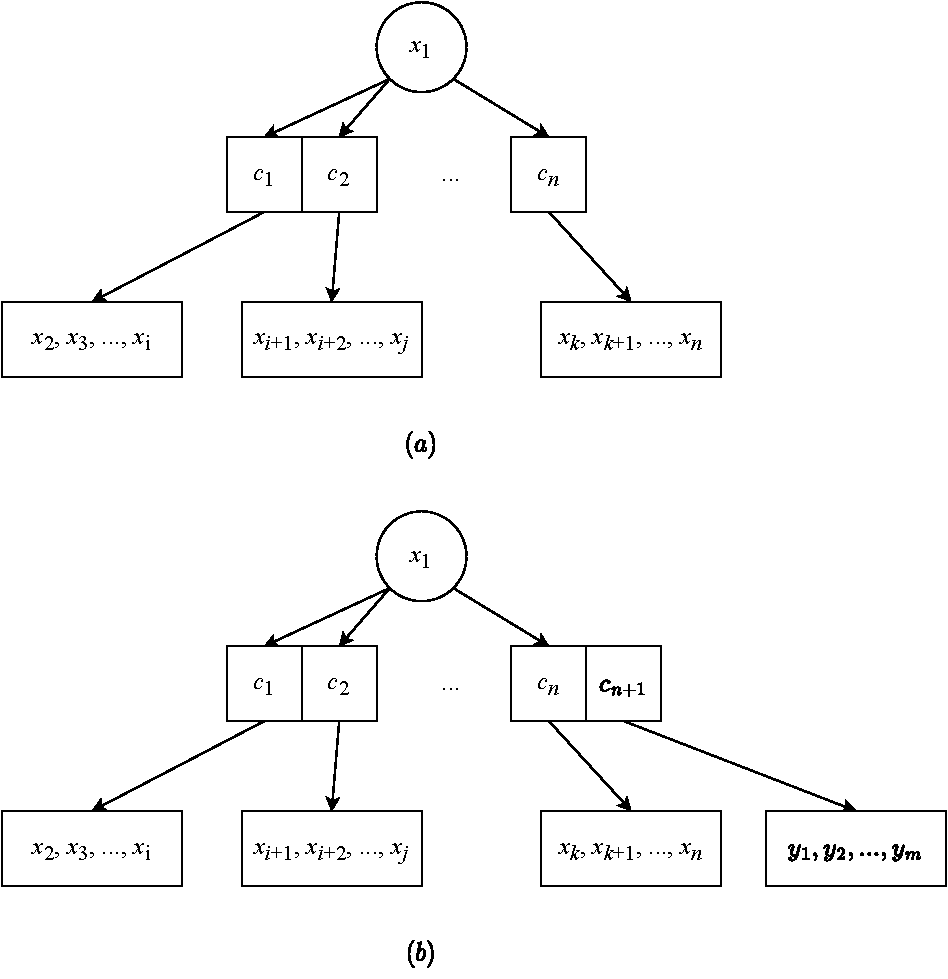
\includegraphics[scale=0.5]{img/clist}} \\
  \subcaptionbox{和另一列表$\{y_1, y_2, ..., y_m\}$连接后的结果}{\includegraphics[scale=0.4]{img/clist1}}
  \caption{可连接列表的数据结构} \label{fig:clist}
\end{figure}

下面的Haskell例子程序定义了这种递归数据结构。

\lstset{language=Haskell}
\begin{lstlisting}[style=Haskell]
data CList a = Empty | CList a (Queue (CList a))
\end{lstlisting}

一个可连接列表或者为空,或者是一个K叉树,包含一个root元素和一个存有$K$棵子树的队列,每棵子树也都是可连接列表。这里我们复用前面章节中定义的实时队列。

设函数$clist(x, Q)$通过一个元素$x$和一个由子列表组成的队列$Q$构造一个可连接列表。函数$root(s)$返回K叉树的根元素,$queue(s)$返回由子序列构成的队列。定义连接算法可以定义如下:

\be
concat(s_1, s_2) =  \left \{
  \begin{array}
  {r@{\quad:\quad}l}
  s_1 & s_2 = \phi \\
  s_2 & s_1 = \phi \\
  clist(x, push(Q, s_2)) & otherwise
  \end{array}
\right .
\ee

其中$x = root(s_1)$、$Q = queue(s_1)$。连接两个列表时,如果任何一个为空,则结果为另一个列表;否则,我们将第二个列表放入第一个列表中队列的尾部。

使用实时队列可以保证入队操作的性能为常数时间$O(1)$,因此列表连接操作的时间为$O(1)$。

下面的Haskell例子程序实现了连接算法。

\begin{lstlisting}[style=Haskell]
concat x Empty = x
concat Empty y = y
concat (CList x q) y = CList x (push q y)
\end{lstlisting}

这一设计既获得了良好的连接操作性能,还同时可以在头部、尾部高效添加元素

\be
cons(x, s) = concat(clist(x, \phi), s)
\ee

\be
append(s, x) = concat(s, clist(x, \phi))
\ee

通过返回K叉树的根,可以获得列表的第一个元素

\be
head(s) = root(s)
\ee

但是从可连接列表的头部删除元素有些复杂。这是因为第一个元素为根节点,删除后我们需要从剩余的子树队列中重新构造一棵K叉树。

根节点被删除后,剩下的所有子树也都是由K叉树表示的可连接列表。我们可以把它们全部连接到一起,形成一个新列表。

\be
concatAll(Q) =  \left \{
  \begin{array}
  {r@{\quad:\quad}l}
  \phi & Q = \phi \\
  concat(front(Q), concatAll(pop(Q))) & otherwise
  \end{array}
\right .
\ee

其中函数$front$返回队列中的第一个元素而不将其删除,而$pop$会执行出队操作。

如果队列为空,说明不存在子树,因此结果为一个空列表;否则,我们将第一棵子树出队,它是一个可连接列表,然后递归地将剩余的子树连接在一起;最后,再把递归连接的结果置于第一棵子树的末尾。

定义好$concatAll$后,我们就可以实现从列表头部删除元素的算法了。

\be
tail(s) = concatAll(queue(s))
\ee

下面的Haskell例子程序实现了这一算法。

\begin{lstlisting}[style=Haskell]
head (CList x _) = x
tail (CList _ q) = concatAll q

concatAll q | isEmptyQ q = Empty
            | otherwise = concat (front q) (concatAll (pop q))
\end{lstlisting}

函数\texttt{isEmptyQ}用来判断一个队列是否为空,它的实现很简单,这里不再赘述。读者可以参考本书附带的例子代码。

算法$concatAll$实际上遍历了队列,逐步归并(reduce)到一个最终的结果。这和我们在二叉搜索树一章中介绍的\underline{fold}概念非常类似。读者可以参考本书的附录了解fold的详细定义和解释。我们可以为队列也定义fold操作\footnote{某些函数式编程语言,例如Haskell,定义了概念为monoid(幺半群)的type class,可以方便地在自定义的数据结构上进行fold。}\cite{learn-haskell}。

\be
foldQ(f, e, Q) = \left \{
  \begin{array}
  {r@{\quad:\quad}l}
  e & Q = \phi \\
  f(front(Q), foldQ(f, e, pop(Q))) & otherwise
  \end{array}
\right .
\ee

函数$foldQ$接受三个参数,一个二元函数$f$,用以reduce,一个初始值$e$,和一个需要遍历的队列$Q$。

我们给出一些在队列上进行fold的例子。假设队列$Q$从头到尾包含元素$\{ 1, 2, 3, 4, 5 \}$。

\[
\begin{array}{l}
foldQ(+, 0, Q) = 1 + (2 + (3 + (4 + (5 + 0)))) = 15 \\
foldQ(\times, 1, Q) = 1 \times (2 \times (3 \times (4 \times (5 \times 1)))) = 120 \\
foldQ(\times, 0, Q) = 1 \times (2 \times (3 \times (4 \times (5 \times 0)))) = 0 \\
\end{array}
\]

仿照这些例子,函数$concatAll$可以用$foldQ$来定义。

\be
concatAll(Q) = foldQ(concat, \phi, Q)
\ee

下面的Haskell例子程序使用fold的概念实现了子树的连接。

\begin{lstlisting}[style=Haskell]
concatAll = foldQ concat Empty

foldQ :: (a -> b -> b) -> b -> Queue a -> b
foldQ f z q | isEmptyQ q = z
            | otherwise = (front q) `f` foldQ f z (pop q)
\end{lstlisting}

但是删除算法的性能并非在所有的情况下都能得到保证。最坏情况发生在用户连续向一个空列表添加$n$个元素后,然后立即执行一次删除时。此时K叉树中,第一个元素存储在根节点,而$n-1$棵子树都只含有一个叶子节点。因此$concatAll$算法退化到线性时间$O(n)$。

元素的插入、添加、删除、以及列表的连接操作如果随机发生,平均下来,这一算法的分摊复杂度是常数时间$O(1)$的。具体证明我们留给读者作为练习。

\begin{Exercise}
\begin{enumerate}
\item 如何将一个元素添加到二叉随机访问列表的末尾?

\item 证明可连接列表的删除操作的分摊复杂度为常数时间$O(1)$,提示:使用banker方法。

\item 选择一门命令式语言,实现可连接列表。
\end{enumerate}
\end{Exercise}

% =========================================
%  Finger tree
% =========================================
\section{手指树(Finger Tree)}
\index{序列!手指树}
我们目前介绍的这些数据结构,尚未达到本章开头给出的全部目标。

二叉随机访问列表可以在头部进行快速地插入、删除,随机访问的速度也比较快。但是两个列表连接的性能不够理想,同时也没有好方法在尾部添加元素。

可连接列表可以快速地将多个列表连接起来,在头部和尾部插入的性能也很好。但是却不支持通过索引随机访问元素。

这两个例子提供了一些思路给我们:

\begin{itemize}
\item 为了能够在头部和尾部进行快速操作,必须能够通过某种方式快速地访问头部和尾部;
\item 类似于树的数据结构可以帮助将随机访问转换成分而治之的搜索,如果树的平衡性很好,则搜索性能可以保证为对数时间。
\end{itemize}

\subsection{定义}
\index{手指树!定义}
手指树(finger tree)\cite{finger-tree-1977}于1977年被提出,可以用于实现高效的序列。并且适于纯函数式的实现\cite{finger-tree-2006}。

我们知道,树的平衡与否,对于搜索的性能至关重要。因此可以考虑使用平衡树作为底层数据结构。手指树的底层数据结构为2-3树,它是一种特殊的B-树(读者可以参考本书前面B树的章节)。

一棵2-3树包含两个或三个子节点。下面的Haskell例子程序定义了2-3树。

\lstset{language=Haskell}
\begin{lstlisting}[style=Haskell]
data Node a = Br2 a a | Br3 a a a
\end{lstlisting}

在命令式编程环境中,节点的定义可以包含一个子节点的列表,这一列表至多包含3个子节点。下面的ANSI C例子程序定义了这样的节点。

\lstset{language=C}
\begin{lstlisting}
union Node {
    Key* keys;
    union Node* children;
};
\end{lstlisting}

这一定义中,一个节点可以包含$2 \sim 3$个key或者$2 \sim 3$棵子树。这里key是叶子节点中元素的类型。

记最左侧的非叶子节点为front手指(也称左侧手指),最右侧的非叶子节点为rear手指(也称右侧手指)。两个手指都是2-3树,并且所有的子节点都是叶子,我们可以直接用含有2到3个叶子的列表表示它们。当然手指树也可以为空,或者是仅含有一个元素的叶子。

归纳起来,一棵手指树可以被描述如下:

\begin{itemize}
\item 一棵手指树或者为空;
\item 或者是仅包含一个元素的叶子;
\item 或者包含三部分:一个左侧手指,是一个至多包含3个元素的列表;一棵子手指树;和一个右侧手指,它也是一个至多包含3个元素的列表。
\end{itemize}

这一定义是递归的,可以容易地用纯函数式的方式实现。下面的Haskell例子程序定义了手指树。

\lstset{language=Haskell}
\begin{lstlisting}[style=Haskell]
data Tree a = Empty
            | Lf a
            | Tr [a] (Tree (Node a)) [a]
\end{lstlisting}

在命令式环境中,我们可以用类似的方法定义手指树。而且,我们还可以增加一个指向parent的变量,方便从任何节点回溯到根节点。下面的ANSI C代码定义了手指树。

\lstset{language=C}
\begin{lstlisting}
struct Tree {
    union Node* front;
    union Node* rear;
    Tree* mid;
    Tree* parent;
};
\end{lstlisting}

我们可以使用空指针NIL代表空树;如果只有一个元素,则将这一元素存储在front手指中。而它的rear手指和中间部分都为空。

图\ref{fig:ftr-example-1}和\ref{fig:ftr-example-2}给出了一些手指树的例子

\begin{figure}[htbp]
  \centering
  \subcaptionbox{空树}{\hspace{0.2\textwidth}\includegraphics[scale=0.5]{img/ftr-empty}\hspace{0.2\textwidth}}
  \subcaptionbox{只含有一个叶子}{\hspace{0.2\textwidth}\includegraphics[scale=0.5]{img/ftr-leaf}\hspace{0.2\textwidth}} \\
  \subcaptionbox{front和rear手指都只含有一个元素,中间部分为空。}{\includegraphics[scale=0.5]{img/ftr-ab}}
  \caption{手指树的例子,1} \label{fig:ftr-example-1}
\end{figure}

\begin{figure}[htbp]
  \centering
  \subcaptionbox{向front手指插入3个元素后,它超过了2-3树的限制,不再平衡。}{\includegraphics[scale=0.5]{img/ftr-abcde}}
  \hspace{0.2\textwidth}
  \subcaptionbox{恢复平衡。front手指含有2个元素;中间部分为一个叶子,包含一棵有3个分支的2-3树。}{\includegraphics[scale=0.5]{img/ftr-abcdef}}
  \caption{手指树的例子,2} \label{fig:ftr-example-2}
\end{figure}

第一个例子为一棵空树;第二个例子是插入一个元素后的结果,变成了只含有一个叶子的节点;第三个例子是含有两个元素的手指树,一个元素在front手指中,另外一个在rear手指中。

如果我们继续向树中插入元素,这些新元素将依次放入front手指中,直到超过2-3树的限制。第四个例子给出了这种情况,front手指中保存了4个元素,树不再平衡。

最后的例子中,树恢复了平衡。front手指中存有2个元素。中间部分不再为空,而是一个含有2-3树的“叶子”(我们稍后解释为什么它是叶子)。叶子的内容为一棵有3个分支的树,每个分支都包含了一个元素。

下面的Haskell表达式对应这5个例子。

\lstset{language=Haskell}
\begin{lstlisting}[style=Haskell]
Empty
Lf a
[b] Empty [a]
[e, d, c, b] Empty [a]
[f, e] Lf (Br3 d c b) [a]
\end{lstlisting}

在最后一个例子中,为什么中间部分的子树是一个叶子呢?手指树的定义是递归的。除去front和rear手指的中间部分是一棵更深的手指树,定义为$Tree(Node(a))$。每当深度增加时,$Node$就会被多嵌入一级。如果第一级的元素类型为$a$,则第二级的元素类型为$Node(a)$,第三级为$Node(Node(a))$……第$n$级为$Node(Node(Node(...(a))...)) = Node^n(a)$,其中$^n$表示$Node$函数被施行(apply)了$n$次。

\subsection{向序列的头部插入元素}
\index{手指树!头部插入}

我们给出的例子实际描述了向手指树逐一插入元素的典型过程。归纳这些例子可以给出在头部插入的算法描述。

当向一棵手指树$T$中插入元素$x$时,
\begin{itemize}
\item 如果树为空,则结果为一个叶子,包含一个元素$x$;
\item 如果树为一个叶子,包含元素$y$,则结果为一棵新手指树。front手指包含了新插入的元素$x$,rear手指包含了此前的元素$y$;中间部分为空的手指树;
\item 如果front手指中包含的元素个数不超过2-3树的上限3,新元素被插入到front手指的最前面;
\item 否则,如果front手指中包含的元素个数超过了2-3树的上限。front手指中的最后3个元素被放入一棵新的2-3树,然后这棵树被递归地插入到中间部分。新元素$x$被插入到front手指中剩余元素的前面。
\end{itemize}

令函数$leaf(x)$创建包含元素$x$的叶子节点,函数$tree(F, T', R)$从三部分构造出一棵手指树:$F$为front手指,是一个包含若干元素的列表。$R$是rear手指;$T'$是中间部分的子树,为一棵更深的手指树。函数$tr3(a, b, c)$从三个元素$a, b, c$创建一棵2-3树;函数$tr2(a, b)$从两个元素$a$和$b$创建一棵2-3树。

\be
insertT(x, T) = \left \{
  \begin{array}
  {r@{\quad:\quad}l}
  leaf(x) & T = \phi \\
  tree(\{x\}, \phi, \{y\}) & T = leaf(y) \\
    \begin{array}{l}
    tree(\{x, x_1\}, insertT( \\
    \quad tr3(x_2, x_3, x_4), T'), R)
    \end{array} &
    \begin{array}{l}
      T = tree(\{x_1, x_2, x_3, x_4\}, \\
      \quad T', R) \end{array} \\
  tree(\{x\} \cup F, T', R) & otherwise
  \end{array}
\right .
\ee

这一算法的性能主要由递归部分决定。其他情况下都是常数时间$O(1)$。递归的深度和树的高度成比例,因此算法的性能为$O(h)$,其中$h$为树的高度。由于使用2-3树并维持平衡,因此$h= O(\lg n)$,其中$n$是手指树中存储元素的个数。

更深入的分析可以给出$insertT$的分摊复杂度为$O(1)$,递归情况消耗的时间可以分摊到其他简单情况中。读者可以参考\cite{okasaki-book}和\cite{finger-tree-2006}来了解详细的证明。

下面的Haskell例子程序实现了插入算法。

\begin{lstlisting}[style=Haskell]
cons :: a -> Tree a -> Tree a
cons a Empty = Lf a
cons a (Lf b) = Tr [a] Empty [b]
cons a (Tr [b, c, d, e] m r) = Tr [a, b] (cons (Br3 c d e) m) r
cons a (Tr f m r) = Tr (a:f) m r
\end{lstlisting}

这段程序使用了LISP的命名传统来描述在如何列表的前面插入元素。

插入算法也可以用命令式的方式实现。设函数\textproc{Tree}()可以构造一棵空树,树中的所有变量包括front手指、rear手指、中间部分子树、和父节点指针都为空。函数\textproc{Node}()用以创建一个空节点。

\begin{algorithmic}
\Function{Prepend-Node}{$n, T$}
  \State $r \gets $ \textproc{Tree}()
  \State $p \gets r$
  \State \Call{Connect-Mid}{$p, T$}
  \While{\textproc{Full?}(\Call{Front}{$T$})}
    \State $F \gets $ \Call{Front}{$T$}  \Comment{$F = \{n_1, n_2, n_3, ...\}$}
    \State \Call{Front}{$T$} $\gets$ $\{n, F[1]\}$  \Comment{$F[1] = n_1$}
    \State $n \gets$ \textproc{Node}()
    \State \Call{Children}{$n$} $\gets F[2..]$  \Comment{$F[2..] = \{ n_2, n_3, ... \}$}
    \State $p \gets T$
    \State $T \gets$ \Call{Mid}{$T$}
  \EndWhile
  \If{$T =$ NIL}
    \State $T \gets$ \textproc{Tree}()
    \State \Call{Front}{$T$}$\gets \{ n \}$
  \ElsIf{ $|$ \Call{Front}{$T$} $|$ = 1 $\land$ \Call{Rear}{$T$} = $\phi$}
    \State \Call{Rear}{$T$} $\gets$ \Call{Front}{$T$}
    \State \Call{Front}{$T$} $\gets \{ n \}$
  \Else
    \State \Call{Front}{$T$} $\gets \{ n \} \cup $ \Call{Front}{$T$}
  \EndIf
  \State \Call{Connect-Mid}{$p, T$} $\gets T$
  \State \Return \Call{Flat}{$r$}
\EndFunction
\end{algorithmic}

其中符号$L[i..]$表示列表$L$的子列表,不包含最前面的$i-1$个元素,若$L = \{a_1, a_2, ..., a_n\}$, 则$L[i..] = \{a_i, a_{i+1}, ..., a_n\}$。

函数\textproc{Front}、\textproc{Rear}、\textproc{Mid}、和\textproc{Parent}分别用以获得front手指、rear手指、中间部分子树、和父节点。函数\textproc{Children}用以获取一个节点的全部子节点。

函数\textproc{Connect-Mid}($T_1, T_2$)将树$T_2$作为中间部分子树连接到$T_1$上。如果$T_2$不为空,还会将$T_1$设置为$T_2$的父节点。

在这一算法中,如果front手指已满,达到3个元素,我们就沿着中间部分子树,进行一次性的自顶向下的遍历。我们将front手指中除第一个元素外的剩余部分抽出,放入一个新节点($Node$深度增加1),然后继续将此新节点插入到中间部分的子树中。front手指剩下原来的第一个元素,待插入元素被放到最前面成为新的第一个元素。

遍历结束后,我们要么到达了一个空树,要么到达了一棵子树,这棵子树的front手指仍然可以容纳更多元素。对于第一种情况,我们创建一个叶子节点,对于后一种情况,我们进行一次简单的列表插入将节点插入到front手指的最前面。

在遍历过程中,我们使用$p$来记录当前树的父节点,这样新创建的树可以被连接到$p$的中间部分作为子树。

最后,我们返回树的根$r$。算法中最后需要解释的是\textproc{Flat}函数。为了简化逻辑,我们创建了一棵空的“ground”树,并让它成为根的父节点。在返回根节点前,我们需要再消除掉这棵多余的“ground”树。这一过程的实现如下:

\begin{algorithmic}
\Function{Flat}{$T$}
  \While{$T \neq$ NIL $\land T$ is empty}
    \State $T \gets$ \Call{Mid}{$T$}
  \EndWhile
  \If{$T \neq$ NIL}
    \State \Call{Parent}{$T$} $\gets $ NIL
  \EndIf
  \State \Return $T$
\EndFunction
\end{algorithmic}

这个while循环用以检查树$T$是否是ground,即树不为NIL($=\phi$),但是front手指和rear手指都是空。

下面的Python例子程序实现了手指树的插入算法。

\lstset{language=Python}
\begin{lstlisting}
def insert(x, t):
    return prepend_node(wrap(x), t)

def prepend_node(n, t):
    root = prev = Tree()
    prev.set_mid(t)
    while frontFull(t):
        f = t.front
        t.front = [n] + f[:1]
        n = wraps(f[1:])
        prev = t
        t = t.mid
    if t is None:
        t = leaf(n)
    elif len(t.front)==1 and t.rear == []:
        t = Tree([n], None, t.front)
    else:
        t = Tree([n]+t.front, t.mid, t.rear)
    prev.set_mid(t)
    return flat(root)

def flat(t):
    while t is not None and t.empty():
        t = t.mid
    if t is not None:
        t.parent = None
    return t
\end{lstlisting}

函数\texttt{set\_mid}、\texttt{frontFull}、\texttt{wrap}、\texttt{wraps}、\texttt{empty}、和树的创建的实现都很简单直观,我们这里不再赘述,读者可以把它们当作练习。

\subsection{从头部删除元素}
\index{手指树!头部删除}

通过把$insertT$中的各个操作进行逆操作,就可以实现从序列头部删除元素。

记$F = \{f_1, f_2, ...\}$为front手指列表,$M$为中间部分子树,$R = \{r_1, r_2, ...\}$为rear手指列表,$R' = \{r_2, r_3, ... \}$为$R$中除去第一个元素外的剩余部分。

\be
extractT(T) = \left \{
  \begin{array}
  {r@{\quad:\quad}l}
  (x, \phi) & T = leaf(x) \\
  (x, leaf(y)) & T = tree(\{x\}, \phi, \{y\}) \\
  (x, tree(\{r_1\}, \phi, R')) & T = tree(\{x\}, \phi, R) \\
  (x, tree(toList(F'), M', R)) &
    \begin{array}{l}
      T = tree(\{x\}, M, R), \\
      (F', M') = extractT(M) \end{array} \\
  (f_1, tree(\{f_2, f_3, ...\}, M, R)) & otherwise
  \end{array}
\right .
\ee

其中函数$toList(T)$将一棵2-3树转换为一个普通列表。如下:

\be
toList(T) = \left \{
  \begin{array}
  {r@{\quad:\quad}l}
  \{x, y\} & T = tr2(x, y) \\
  \{x, y, z\} & T = tr3(x, y, z)
  \end{array}
\right .
\ee

我们略过了错误处理(例如从一个空树中删除元素的错误)。如果手指树是只包含一个元素的叶子,则删除的结果为一棵空树;如果手指树包含两个元素,一个元素在front手指,另一个元素在rear手指,我们删除front手指中的元素,结果变成了只含有一个元素的叶子;如果front手指中只含有一个元素,中间部分为空,而rear手指不空,我们删除front手指中的唯一元素,然后从rear手指中“借”一个元素放入front手指;如果front手指只有一个元素,而中间部分的子树不为空,我们就递归地从子树中删除一个节点,然后将这一节点转换成普通列表来代替front手指。而原来front手指中的唯一元素被删除并返回;最后一种情况,如果front手指包含一个以上的元素,我们只需要将第一个元素删除,而维持其它部分不变。

\begin{figure}[htbp]
  \centering
  \subcaptionbox{用手指树表示的含有10个元素的序列。}{\includegraphics[scale=0.4]{img/ftr-10}} \\
  \subcaptionbox{删除第一个元素后,front手指还剩一个元素。}{\includegraphics[scale=0.4]{img/ftr-9}} \\
  \subcaptionbox{再次从头部删除一个元素,我们从中间部分的子树“借”一个节点,将这个节点从一棵2-3树转换成一个列表,作为新的front手指。中间部分的子树变成了含有一棵2-3树节点的叶子。}{\hspace{0.2\textwidth}\includegraphics[scale=0.4]{img/ftr-8}\hspace{0.2\textwidth}}
  \caption{从一个序列的头部依次删除两个元素的例子} \label{fig:ftr-uncons-example}
\end{figure}

图\ref{fig:ftr-uncons-example}展示了从序列头部删除两个元素的例子。手指树中存有10个元素。当第一个元素被删除后,front手指中还剩一个元素。接着再次删除一个元素后,front手指变为空。我们从中间的子树中“借”一个节点。把它从一棵2-3树转换成含有3个元素的列表。这一列表成为新的front手指。中间部分的子树从原来的三部分变成一个只含有一个2-3树节点的叶子。这一节点包含三个元素。

下面的Haskell例子程序实现了\texttt{uncons}。

\lstset{language=Haskell}
\begin{lstlisting}[style=Haskell]
uncons :: Tree a -> (a, Tree a)
uncons (Lf a) = (a, Empty)
uncons (Tr [a] Empty [b]) = (a, Lf b)
uncons (Tr [a] Empty (r:rs)) = (a, Tr [r] Empty rs)
uncons (Tr [a] m r) = (a, Tr (nodeToList f) m' r) where (f, m') = uncons m
uncons (Tr f m r) = (head f, Tr (tail f) m r)
\end{lstlisting}

其中函数\texttt{nodeToList}定义如下:

\begin{lstlisting}[style=Haskell]
nodeToList :: Node a -> [a]
nodeToList (Br2 a b) = [a, b]
nodeToList (Br3 a b c) = [a, b, c]
\end{lstlisting}

类似地,我们可以使用\texttt{uncons}定义函数\texttt{head}和\texttt{tail}。

\begin{lstlisting}[style=Haskell]
head = fst . uncons
tail = snd . uncons
\end{lstlisting}

\subsection{删除时处理不规则的手指树}
\index{手指树!不规则的手指树}
删除的算法可以归纳为“删除——借”策略。如果删除后front手指变空,就从中间部分的子树中“借”节点。但是树的形式有可能是不规则的,例如front手指和中间子树都为空。这种情况通常是由于分拆操作造成的,我们稍后会详细介绍。

\begin{figure}[htbp]
  \centering
  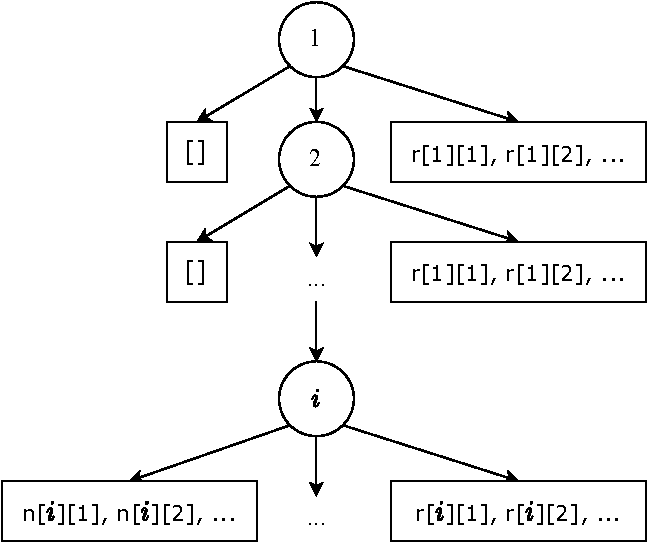
\includegraphics[scale=0.4]{img/ftr-illed-1}
  \caption{不规则树的例子,第$i$层子树的front手指不为空} \label{fig:ftr-illed-form}
\end{figure}

我们要设计一个命令式算法,可以从不规则的手指树中删除第一个元素。思路是首先进行一轮自顶向下的遍历,找到一棵子树,或者它的front手指不为空,或者它的front手指和中间部分的子树都为空,如图\ref{fig:ftr-illed-form}。对于前者,我们可以从front手指中提取出第一个元素,它为一个节点。对于后者,由于只有rear手指不为空,我们可以把它和空的front手指交换,将其转换成前一种情况。

此后,我们需要检查从front手指中取出的节点是否为叶子节点(如何做到?我们将这一问题留给读者作为练习),如果不是,我们需要继续从这一节点的子节点中提取出第一个子节点,而把剩余的节点列表作为当前树的父节点的front手指。我们需要沿着父节点一直向上回溯,直到我们提取到一个叶子节点。此时我们将到达树的根节点。图\ref{fig:ftr-illed-extract}描述了这一过程。

\begin{figure}[htbp]
  \centering
  \subcaptionbox{提取第一个元素n{[i]}{[1]},然后将它的子节点放到上一级树的front手指中。}{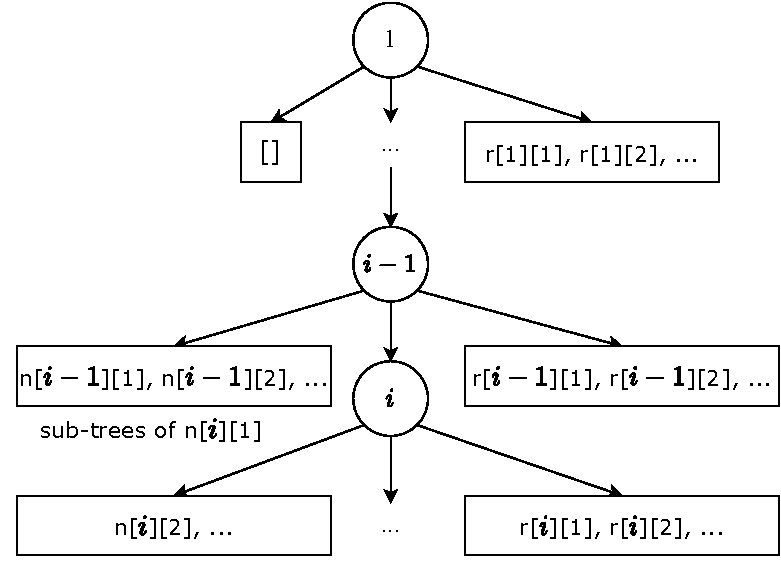
\includegraphics[scale=0.4]{img/ftr-illed-2}}
  \subcaptionbox{重复这一过程$i$次,最终提取到x{[1]}。}{\hspace{0.1\textwidth}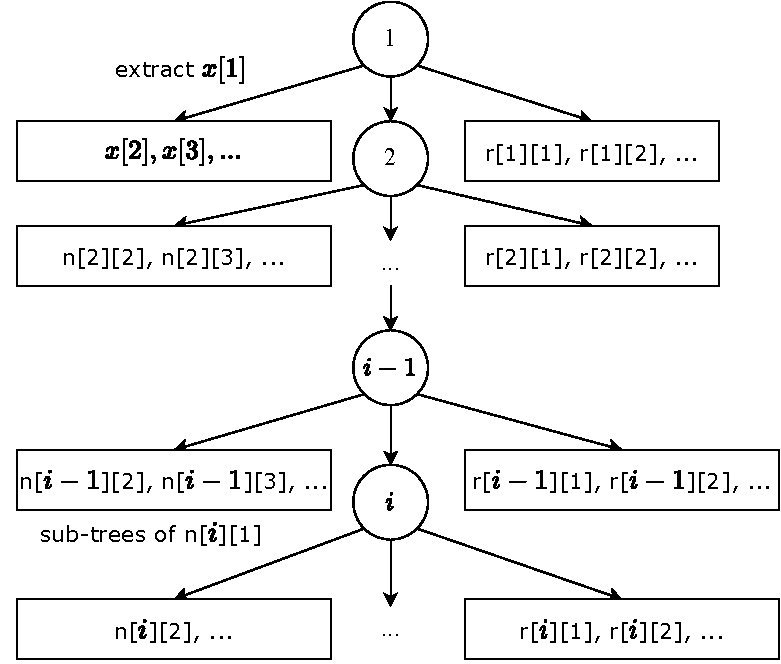
\includegraphics[scale=0.4]{img/ftr-illed-i}}
  \caption{自底向上遍历,直到提取出一个叶子节点} \label{fig:ftr-illed-extract}
\end{figure}

根据这一思路,下面的算法实现了列表头部的删除操作。这里假设传入的树不为空。

\begin{algorithmic}
\Function{Extract-Head}{$T$}
  \State $r \gets$ \textproc{Tree}()
  \State \Call{Connect-Mid}{$r, T$}
  \While{\Call{Front}{$T$} $= \phi \land $ \Call{Mid}{$T$} $\neq $ NIL}
    \State $T \gets$ \Call{Mid}{$T$}
  \EndWhile

  \If{\Call{Front}{$T$} $ = \phi \land $ \Call{Rear}{$T$} $\neq \phi$}
    \State \textproc{Exchange} \Call{Front}{$T$} $\leftrightarrow$ \Call{Rear}{$T$}
  \EndIf

  \State $n \gets $ \textproc{Node}()
  \State \Call{Children}{$n$} $\gets$ \Call{Front}{$T$}
  \Repeat
    \State $L \gets$ \Call{Children}{$n$} \Comment{$L = \{n_1, n_2, n_3, ...\}$}
    \State $n \gets L[1]$ \Comment{$ n \gets n_1$}
    \State \Call{Front}{$T$} $\gets L[2..]$ \Comment{$L[2..] = \{n_2, n_3, ...\}$}
    \State $T \gets $ \Call{Parent}{$T$}
    \If{\Call{Mid}{$T$} becomes empty}
      \State \Call{Mid}{$T$} $\gets$ NIL
    \EndIf
  \Until{$n$ is a leaf}
  \State \Return (\Call{Elem}{$n$}, \Call{Flat}{$r$})
\EndFunction
\end{algorithmic}

这里函数\textproc{Elem}($n$)返回叶子节点$n$中保存的唯一元素。和命令式插入算法类似,这里使用了一棵“ground”树作为根节点的父节点。这样可以简化边界处理的逻辑。因此最后在返回前要做额外的处理,去除掉多余的“grand”树。

下面的Python例子程序实现了这一算法。

\lstset{language=Python}
\begin{lstlisting}
def extract_head(t):
    root = Tree()
    root.set_mid(t)
    while t.front == [] and t.mid is not None:
        t = t.mid
    if t.front == [] and t.rear != []:
        (t.front, t.rear) = (t.rear, t.front)
    n = wraps(t.front)
    while True: # repeat-until循环
        ns = n.children
        n = ns[0]
        t.front = ns[1:]
        t = t.parent
        if t.mid.empty():
            t.mid.parent = None
            t.mid = None
        if n.leaf:
            break
    return (elem(n), flat(root))
\end{lstlisting}

如果树的front手指和rear手指都为空,则成员函数\texttt{Tree.empty()}返回真。我们增加了一个标记\texttt{Node.leaf}来记录一个节点是叶子节点,还是复合节点。本节的练习要求读者思考其他的方法。

由于允许不规则的树存在,从手指树中获取第一个和最后一个元素的算法需要做相应的调整,对于不规则的树,手指可以为空,我们不再仅仅返回手指的第一个或者最后一个子节点。

解决方法和\textproc{Extract-Head}类似,如果手指为空,而中间部分的子树不为空,我们就沿着中间部分向下遍历,直到发现手指不为空,或者所有的节点都存储在另一侧的手指中。例如下面的算法,即使是不规则树,也能返回第一个叶子节点。

\begin{algorithmic}
\Function{First-Lf}{$T$}
  \While{\Call{Front}{$T$} $ = \phi \land $ \Call{Mid}{$T$} $\neq$ NIL}
    \State $T \gets$ \Call{Mid}{$T$}
  \EndWhile
  \If{\Call{Front}{$T$} $ = \phi \land$ \Call{Rear}{$T$} $\neq \phi$}
    \State $n \gets$ \Call{Rear}{$T$}[1]
  \Else
    \State $n \gets$ \Call{Front}{$T$}[1]
  \EndIf
  \While{$n$ is NOT leaf}
    \State $n \gets$ \Call{Children}{$n$}[1]
  \EndWhile
  \State \Return $n$
\EndFunction
\end{algorithmic}

注意其中的第二个循环,如果当前的节点不是叶子,它就不断沿着第一个子节点遍历。最后我们会得到一个叶子节点,从而可以获取到元素。

\begin{algorithmic}
\Function{First}{$T$}
  \State \Return \textproc{Elem}(\Call{First-Lf}{$T$})
\EndFunction
\end{algorithmic}

下面的Python例子程序实现了这一算法。

\lstset{language=Python}
\begin{lstlisting}
def first(t):
    return elem(first_leaf(t))

def first_leaf(t):
    while t.front == [] and t.mid is not None:
        t = t.mid
    if t.front == [] and t.rear != []:
        n = t.rear[0]
    else:
        n = t.front[0]
    while not n.leaf:
        n = n.children[0]
    return n
\end{lstlisting}

获取最后一个元素与此类似,我们将其作为练习留给读者。

\subsection{在序列的尾部添加元素}
\index{手指树!尾部添加}

由于手指树是对称的,我们可以参考$insertT$实现尾部添加算法。

\be
appendT(T, x) = \left \{
  \begin{array}
  {r@{\quad:\quad}l}
  leaf(x) & T = \phi \\
  tree(\{y\}, \phi, \{x\}) & T = leaf(y) \\
  \begin{array}{l}
  tree(F, \\
  appendT(M, tr3(x_1, x_2, x_3)), \\
  \{x_4, x\}) \end{array} &
    \begin{array}{l} T = tree(F, M, \\
    \{x_1, x_2, x_3, x_4\}) \end{array} \\
  tree(F, M, R \cup \{x\}) & otherwise
  \end{array}
\right .
\ee

如果rear手指仍然是合法的2-3树,包含的元素不超过4个,新元素就可以直接插入到rear手指中。否则,我们将rear手指分拆,将前三个元素取出,构造一棵新的2-3树,递归地添加到中间部分子树的末尾。此外,我们还要处理两种边界情况:一种是手指树为空,另外一种是仅含有一个叶子节点。

下面的Haskell例子程序实现了尾部添加算法。

\lstset{language=Haskell}
\begin{lstlisting}[style=Haskell]
snoc :: Tree a -> a -> Tree a
snoc Empty a = Lf a
snoc (Lf a) b = Tr [a] Empty [b]
snoc (Tr f m [a, b, c, d]) e = Tr f (snoc m (Br3 a b c)) [d, e]
snoc (Tr f m r) a = Tr f m (r++[a])
\end{lstlisting}

函数的名字\texttt{snoc}恰好是\texttt{cons}倒过来,我们以此指出它们操作上的对称关系。

用命令式的方法在尾部添加元素与此类似,下面的算法实现了这一操作。

\begin{algorithmic}
\Function{Append-Node}{$T, n$}
  \State $r \gets $ \textproc{Tree}()
  \State $p \gets r$
  \State \Call{Connect-Mid}{$p, T$}
  \While{\textproc{Full?}(\Call{Rear}{$T$})}
    \State $R \gets $ \Call{Rear}{$T$} \Comment{$R = \{n_1, n_2, ..., , n_{m-1}, n_m \}$}
    \State \Call{Rear}{$T$} $\gets$ $\{n, $ \Call{Last}{$R$} $\}$ \Comment{last element $n_m$}
    \State $n \gets$ \textproc{Node}()
    \State \Call{Children}{$n$} $\gets R[1...m-1]$ \Comment{ $\{n1, n2, ..., n_{m-1}\}$}
    \State $p \gets T$
    \State $T \gets$ \Call{Mid}{$T$}
  \EndWhile
  \If{$T =$ NIL}
    \State $T \gets$ \textproc{Tree}()
    \State \Call{Front}{$T$} $\gets \{ n \}$
  \ElsIf{ $|$ \Call{Rear}{$T$} $|$ = 1 $\land$ \Call{Front}{$T$} = $\phi$}
    \State \Call{Front}{$T$} $\gets$ \Call{Rear}{$T$}
    \State \Call{Rear}{$T$} $\gets \{ n \}$
  \Else
    \State \Call{Rear}{$T$} $\gets$ \Call{Rear}{$T$} $\cup \{ n \} $
  \EndIf
  \State \Call{Connect-Mid}{$p, T$} $\gets T$
  \State \Return \Call{Flat}{$r$}
\EndFunction
\end{algorithmic}

对应的Python例子程序如下。

\lstset{language=Python}
\begin{lstlisting}
def append_node(t, n):
    root = prev = Tree()
    prev.set_mid(t)
    while rearFull(t):
        r = t.rear
        t.rear = r[-1:] + [n]
        n = wraps(r[:-1])
        prev = t
        t = t.mid
    if t is None:
        t = leaf(n)
    elif len(t.rear) == 1 and t.front == []:
        t = Tree(t.rear, None, [n])
    else:
        t = Tree(t.front, t.mid, t.rear + [n])
    prev.set_mid(t)
    return flat(root)
\end{lstlisting}

\subsection{从尾部删除元素}
\index{手指树!尾部删除}

和$appendT$类似,我们可以通过实现$extractT$的逆操作从尾部删除最后一个元素。

记非空、非单一叶子的手指树为$tree(F, M, R)$,其中$F$为front手指,$M$为中间部分的子树,$R$为rear手指。

\be
removeT(T) = \left \{
  \begin{array}
  {r@{\quad:\quad}l}
  (\phi, x) & T = leaf(x) \\
  (leaf(y), x) & T = tree(\{y\}, \phi, \{x\}) \\
  (tree(init(F), \phi, last(F)), x) & T = tree(F, \phi, \{x\}) \land F \neq \phi \\
  (tree(F, M', toList(R')), x) & \begin{array}{l}
  T = tree(F, M, \{x\}), \\
  (M', R') = removeT(M) \end{array} \\
  (tree(F, M, init(R)), last(R)) & otherwise
  \end{array}
\right .
\ee

函数$toList(T)$的定义和此前一样,它将一棵2-3树转换为普通列表。函数$init(L)$返回列表$L$中除最后一个元素外的剩余部分,若$L = \{a_1, a_2, ..., a_{n-1}, a_n\}$,则$init(L) = \{a_1, a_2, ..., a_{n-1}\}$。函数$last(L)$返回列表$L$中的最后一个元素,即$last(L) = a_n$。读者可以参考本书的附录了解它们的具体实现。

下面的Haskell例子程序实现了尾部删除算法。函数被命名为\texttt{unsnoc}以表明它是函数\texttt{snoc}的逆运算。

\lstset{language=Haskell}
\begin{lstlisting}[style=Haskell]
unsnoc :: Tree a -> (Tree a, a)
unsnoc (Lf a) = (Empty, a)
unsnoc (Tr [a] Empty [b]) = (Lf a, b)
unsnoc (Tr f@(_:_) Empty [a]) = (Tr (init f) Empty [last f], a)
unsnoc (Tr f m [a]) = (Tr f m' (nodeToList r), a) where (m', r) = unsnoc m
unsnoc (Tr f m r) = (Tr f m (init r), last r)
\end{lstlisting}

我们也可以为手指树定义类似列表的\texttt{last}和\texttt{init}函数。

\begin{lstlisting}[style=Haskell]
last = snd . unsnoc
init = fst . unsnoc
\end{lstlisting}

命令式的尾部删除算法和头部删除类似。但是这里存在一个特殊情况,当只有一个元素(或者子节点)时,我们总是将其存储在front手指,而rear手指和中间部分的子树为空(即:$Tree(\{n\}, NIL, \phi)$),如果只从rear手指获取最后一个元素,就无法得到正确的结果。

如果rear手指为空,这一特殊情况可以通过交换front手指和rear手指来解决,如下面的算法所示:

\begin{algorithmic}
\Function{Extract-Tail}{$T$}
  \State $r \gets$ \textproc{Tree}()
  \State \Call{Connect-Mid}{$r, T$}
  \While{\Call{Rear}{$T$} $= \phi \land $ \Call{Mid}{$T$} $\neq $ NIL}
    \State $T \gets$ \Call{Mid}{$T$}
  \EndWhile

  \If{\Call{Rear}{$T$} $ = \phi \land $ \Call{Front}{$T$} $\neq \phi$}
    \State \textproc{Exchange} \Call{Front}{$T$} $\leftrightarrow$ \Call{Rear}{$T$}
  \EndIf

  \State $n \gets $ \textproc{Node}()
  \State \Call{Children}{$n$} $\gets$ \Call{Rear}{$T$}
  \Repeat
    \State $L \gets$ \Call{Children}{$n$} \Comment{$L = \{n_1, n_2, ..., n_{m-1}, n_m\}$}
    \State $n \gets$ \Call{Last}{$L$} \Comment{$ n \gets n_m$}
    \State \Call{Rear}{$T$} $\gets L[1...m-1]$ \Comment{$\{n_1, n_2, ..., n_{m-1}\}$}
    \State $T \gets $ \Call{Parent}{$T$}
    \If{\Call{Mid}{$T$} becomes empty}
      \State \Call{Mid}{$T$} $\gets$ NIL
    \EndIf
  \Until{$n$ is a leaf}
  \State \Return (\Call{Elem}{$n$}, \Call{Flat}{$r$})
\EndFunction
\end{algorithmic}

我们把如何获得最后一个元素,以及这一算法的实现留给读者作为练习。

\subsection{连接}
\index{手指树!连接}

考虑两棵手指树都不为空的情况。记两棵树为$T_1 = tree(F_1, M_1, R_1)$和$T_2 = tree(F_2, M_2, R_2)$。可以用$F_1$作为连接结果的新front手指,用$R_2$作为连接结果的新rear手指。我们需要将$M_1$、$R_1$、$F_2$、$M_2$合并成一棵新的中间部分子树。

由于$R_1$和$F_2$都是节点的列表,所以这一问题等价于实现如下的算法:

\[
merge(M_1, R_1 \cup F_2, M_2) = ?
\]

进一步观察可以发现,$M_1$和$M_2$都是手指树,只不过它们比$T_1$和$T_2$的节点深度大一级,若$T_1$树中存储的元素类型为$a$,则$M_1$中存储的元素类型为$Node(a)$。因此,我们可以递归地进行合并:保留$M_1$的front手指和$M_2$的rear手指,然后将$M_1$和$M_2$的中间部分,以及$M_1$的rear手指和$M_2$的front手指合并。

记函数$front(T)$返回树$T$的front手指,$rear(T)$返回rear手指,$mid(T)$返回中间部分的子树。当两棵树都不为空时,$merge$算法可以定义如下:

\be
\begin{array}{l}
merge(M_1, R_1 \cup F_2, M_2) = tree(front(M_1), S, rear(M_2)) \\
S = merge(mid(M_1), rear(M_1) \cup R_1 \cup F_2 \cup front(M_2), mid(M_2))
\end{array}
\label{eq:merge-recursion}
\ee

而树的连接算法也可以使用$merge()$来定义。

\be
concat(T_1, T_2) = tree(F_1, merge(M_1, R_1 \cup F_2, M_2), R_2)
\ee

比较这一定义和式(\ref{eq:merge-recursion}),我们发现连接操作本质上就是合并操作,我们可以给出下面的定义:

\be
concat(T_1, T_2) = merge(T_1, \phi, T_2)
\ee

最后,我们需要为$merge()$算法定义边界条件。

\be
merge(T_1, S, T_2) =  \left \{
  \begin{array}
  {r@{\quad:\quad}l}
  foldR(insertT, T_2, S) & T_1 = \phi \\
  foldL(appendT, T_1, S) & T_2 = \phi \\
  merge(\phi, \{x\} \cup S, T_2) & T_1 = leaf(x) \\
  merge(T_1, S \cup \{x\}, \phi) & T_2 = leaf(x) \\
  \begin{array}{l}
  tree(F_1, merge(M_1, \\
  \quad nodes(R_1 \cup S \cup F_2), M2), R_2) \end{array} & otherwise
  \end{array}
\right .
\ee

大部分的情况都比较直观。若$T_1$或$T_2$中的任何一棵为空,算法就逐一将列表$S$中的元素插入或者添加到另一棵树中;函数$foldL$和$foldR$类似于命令式编程环境中的for-each循环。其中$foldL$自左向右处理$S$中的元素,而$foldR$自右向左处理。

对于非空列表$L=\{ a_1, a_2, ..., a_{n-1}, a_n\}$,记$L' = \{ a_2, a_3, ..., a_{n-1}, a_n\}$为除第一元素外的剩余部分。$foldL$和$foldR$可以分别定义如下:

\be
foldL(f, e, L) = \left \{
  \begin{array}
  {r@{\quad:\quad}l}
  e & L = \phi \\
  foldL(f, f(e, a_1), L') & otherwise
  \end{array}
\right .
\ee

\be
foldR(f, e, L) = \left \{
  \begin{array}
  {r@{\quad:\quad}l}
  e & L = \phi \\
  f(a_1, foldR(f, e, L')) & otherwise
  \end{array}
\right .
\ee

读者可以参考本书的附录了解它们的详细内容。

若任一棵树是仅包含一个元素的叶子,我们将这一元素插入或者添加到$S$中将其转换为前一种边界情况(其中一棵树为空的情况)。

函数$nodes$将元素列表转换成一组2-3树的列表。这是因为中间部分的子树中的元素类型,比手指中的元素类型在$Node$上深一级。考虑递归调用达到边界情况的时候,假设此时$M_1$为空,我们需要逐一将所有$R_1 \cup S \cup F_2$中的元素插入$M_2$。但是我们不能直接执行插入操作,若此时的元素类型为$a$,我们只能将类型为2-3树的$Node(a)$插入到$M_2$中。这和前面的$insertT$算法中的处理类似:取出最后三个元素,转换成一棵2-3树,然后递归地执行$insertT$。下面给出了$nodes$的定义:

\be
nodes(L) = \left \{
  \begin{array}
  {r@{\quad:\quad}l}
  \{tr2(x_1, x_2)\} & L = \{x_1, x_2\} \\
  \{tr3(x_1, x_2, x_3)\} & L = \{x_1, x_2, x_3\} \\
  \{tr2(x_1, x_2), tr2(x_3, x_4)\} & L = \{x_1, x_2, x_3, x_4\} \\
  \{tr3(x_1, x_2, x_3)\} \cup nodes(\{x_4, x_5, ...\}) & otherwise
  \end{array}
\right .
\ee

函数$nodes$需要遵守2-3树的限制条件,若列表中只有2个或3个元素,结果是只含有一棵2-3树的列表;若列表中含有4个元素,则结果列表中包含两棵树,每棵树有两个分支;否则,如果多于4个元素,就将前3个元素放到一棵2-3树中,然后递归地调用$nodes$来处理剩余的元素。

连接操作的性能取决于合并算法。分析递归的情况可以发现,递归的深度和两棵树种较矮的一棵成比例。由于2-3树可以保证平衡性,它的高度为$O(\lg n')$其中$n'$为元素的个数。合并在边界条件下的性能和插入一样(最多调用$insertT$8次)为分摊时间$O(1)$,最坏情况问为$O(\lg m)$,其中$m$是两棵树的高度差。因此,总体上算法的复杂度为$O(\lg n)$,其中$n$是两棵手指树中含有的元素总数。

下面的Haskell例子程序实现了连接算法

\lstset{language=Haskell}
\begin{lstlisting}[style=Haskell]
concat :: Tree a -> Tree a -> Tree a
concat t1 t2 = merge t1 [] t2
\end{lstlisting}

由于Haskell标准库prelude中含有一个名为\texttt{concat}的函数,因此需要做一些额外的处理,如隐藏import或者更换名字,以避免冲突。

\begin{lstlisting}[style=Haskell]
merge :: Tree a -> [a] -> Tree a -> Tree a
merge Empty ts t2 = foldr cons t2 ts
merge t1 ts Empty = foldl snoc t1 ts
merge (Lf a) ts t2 = merge Empty (a:ts) t2
merge t1 ts (Lf a) = merge t1 (ts++[a]) Empty
merge (Tr f1 m1 r1) ts (Tr f2 m2 r2) = Tr f1 (merge m1 (nodes (r1 ++ ts ++ f2)) m2) r2
\end{lstlisting}

其中$nodes$函数的实现如下:

\begin{lstlisting}[style=Haskell]
nodes :: [a] -> [Node a]
nodes [a, b] = [Br2 a b]
nodes [a, b, c] = [Br3 a b c]
nodes [a, b, c, d] = [Br2 a b, Br2 c d]
nodes (a:b:c:xs) = Br3 a b c:nodes xs
\end{lstlisting}

为了用命令式的方式连接两棵手指树$T_1$和$T_2$,我们需要沿着两棵树的中间部分的子树向下遍历,直到其中一棵为空。每次迭代中,我们创建一棵新树,用$T_1$的front手指作为新树$T$的front手指;用$T_2$的rear手指作为$T$的rear手指。剩下的两个手指($T_1$的rear手指和$T_2$的front手指)中的元素被放入一个列表,然后被分组放入若干2-3树中。记这一2-3树的列表为$N$。$N$不仅随着遍历在长度上增加,而且每次迭代元素的深度也增加一级。我们将这棵新树附加到上一级的树中作为中间部分,然后进入下一次迭代。

当两棵树种的任一棵树变为空的时候,我们停止遍历,然后逐一将$N$中的2-3树插入到另一棵非空的树中,并将其设为上一级结果的中间部分子树。

下面的算法给出了这一过程的详细描述。

\begin{algorithmic}
\Function{Concat}{$T_1, T_2$}
  \State \Return \Call{Merge}{$T_1, \phi, T_2$}
\EndFunction
\Statex
\Function{Merge}{$T_1, N, T_2$}
  \State $r \gets$ \textproc{Tree}()
  \State $p \gets r$

  \While{$T_1 \neq$ NIL $\land T_2 \neq$ NIL}
    \State $T \gets$ \textproc{Tree}()
    \State \Call{Front}{$T$} $\gets$ \Call{Front}{$T_1$}
    \State \Call{Rear}{$T$} $\gets$ \Call{Rear}{$T_2$}
    \State \Call{Connect-Mid}{$p, T$}
    \State $p \gets T$
    \State $N \gets$ \textproc{Nodes}(\Call{Rear}{$T_1$} $\cup N \cup$ \Call{Front}{$T_2$})
    \State $T_1 \gets$ \Call{Mid}{$T_1$}
    \State $T_2 \gets$ \Call{Mid}{$T_2$}
  \EndWhile

  \If{$T_1 =$ NIL}
    \State $T \gets T_2$
    \For{each $n \in $ \Call{Reverse}{$N$}}
      \State $T \gets$ \Call{Prepend-Node}{$n, T$}
    \EndFor
  \ElsIf{$T_2 =$ NIL}
    \State $T \gets T_1$
    \For{each $n \in N$}
      \State $T \gets$ \Call{Append-Node}{$T, n$}
    \EndFor
  \EndIf
  \State \Call{Connect-Mid}{$p, T$}

  \State \Return \Call{Flat}{$r$}
\EndFunction
\end{algorithmic}

算法中的for-each循环也可以用左侧fold或者右侧fold来实现。下面的Python例子程序实现了这一算法。

\lstset{language=Python}
\begin{lstlisting}
def concat(t1, t2):
    return merge(t1, [], t2)

def merge(t1, ns, t2):
    root = prev = Tree() #作为哨兵的dummy节点
    while t1 is not None and t2 is not None:
        t = Tree(t1.size + t2.size + sizeNs(ns), t1.front, None, t2.rear)
        prev.set_mid(t)
        prev = t
        ns = nodes(t1.rear + ns + t2.front)
        t1 = t1.mid
        t2 = t2.mid
    if t1 is None:
        prev.set_mid(foldR(prepend_node, ns, t2))
    elif t2 is None:
        prev.set_mid(reduce(append_node, ns, t1))
    return flat(root)
\end{lstlisting}

由于Python标准库只提供了左侧fold的函数\texttt{reduce},右侧fold可以按照下面的定义实现,逐一将元素按照逆序取出并应用传入的函数。

\begin{lstlisting}
def foldR(f, xs, z):
    for x in reversed(xs):
        z = f(x, z)
    return z
\end{lstlisting}

唯一需要实现的算法是将若干元素平衡分组放入一些2-3树中。一棵2-3树最多可以容纳3个分支,若元素个数多于4,我们可以取出3个放入一棵树中,然后继续处理剩下的元素。若只含有4个,则它们被分成2棵2个分支的树。对于其余的情况(3个、2个或1个),我们将它们全部放入一棵2-3树中。

记节点列表为$L=\{ n_1, n_2, ... \}$,下面的算法实现了这一处理过程。

\begin{algorithmic}
\Function{Nodes}{$L$}
  \State $N = \phi$
  \While{$|L| > 4$}
    \State $n \gets$ \textproc{Node}()
    \State \Call{Children}{$n$} $\gets L[1..3]$  \Comment{ $\{n_1, n_2, n_3 \}$ }
    \State $N \gets N \cup \{ n \}$
    \State $L \gets L[4...]$ \Comment{ $\{ n_4, n_5, ... \}$ }
  \EndWhile

  \If{$|L| = 4$}
    \State $x \gets$ \textproc{Node}()
    \State \Call{Children}{$x$} $\gets \{L[1], L[2]\}$
    \State $y \gets$ \textproc{Node}()
    \State \Call{Children}{$y$} $\gets \{L[3], L[4]\}$
    \State $N \gets N \cup \{ x, y \}$
  \ElsIf{$L \neq \phi$}
    \State $n \gets$ \textproc{Node}()
    \State \Call{Children}{$n$} $\gets L$
    \State $N \gets N \cup \{ n \}$
  \EndIf

  \State \Return $N$
\EndFunction
\end{algorithmic}

下面的Python例子程序实现了这一算法,其中函数\texttt{wraps()}首先创建一棵树,然后将一个列表中的元素设为节点的子树。

\begin{lstlisting}
def nodes(xs):
    res = []
    while len(xs) > 4:
        res.append(wraps(xs[:3]))
        xs = xs[3:]
    if len(xs) == 4:
        res.append(wraps(xs[:2]))
        res.append(wraps(xs[2:]))
    elif xs != []:
        res.append(wraps(xs))
    return res
\end{lstlisting}

\begin{Exercise}
\begin{enumerate}
\item 选择一门命令式语言,实现完整的手指树插入算法。

\item 如何判定一个节点是否是叶子?它仅包含一个基本元素还是包含一个含有若干子树的复合节点?我们不能仅仅通过size来进行判定,例如只包含一个叶子的节点,形如$node(1, \{node(1, \{x\}\})$。请分别使用动态类型语言(如Python或lisp)和静态类型语言(如C++)来解决这一问题。

\item 选择一门命令式语言,实现\textproc{Extract-Tail}算法。

\item 分别用函数式和命令式的方法返回一棵手指树中的最后一个元素,对于命令式方法,要求能够处理不规则树。

\item 不使用fold,实现手指树的连接算法。可以使用递归或者循环。
\end{enumerate}
\end{Exercise}

\subsection{手指树的随机访问}
\index{手指树!随机访问}

\subsubsection{增加size记录}
\index{手指树!size记录}
提供快速随机访问的策略是将其转换为树搜索。为了避免反复计算树的size,我们给树和节点增加size变量。

下面的Haskell例子代码在定义中增加了size信息。

\lstset{language=Haskell}
\begin{lstlisting}[style=Haskell]
data Tree a = Empty
            | Lf a
            | Tr Int [a] (Tree (Node a)) [a]
\end{lstlisting}

下面的ANSI C结构定义中也增加了size信息。

\lstset{language=C}
\begin{lstlisting}
struct Tree {
    union Node* front;
    union Node* rear;
    Tree* mid;
    Tree* parent;
    int size;
};
\end{lstlisting}

设函数$tree(s, F, M, R)$从size信息$s$、front手指列表$F$、rear手指列表$R$、和中间部分的子树$M$构造一棵手指树。当我们需要获得size信息时,可以通过函数$size(T)$来获取:

\[
size(T) = \left \{
  \begin{array}
  {r@{\quad:\quad}l}
  0 & T = \phi \\
  ? & T = leaf(x) \\
  s & T = tree(s, F, M, R)
  \end{array}
\right .
\]

若树为空,则size为0;若树可以表示为$tree(s, F, M, R)$则size为$s$;但是当树只有一片叶子时他的size是什么?它是1么?答案是否定的。只有当$T = leaf(a)$并且$a$不是一个节点而是一个元素时size才等于1。其余情况下,size都不为1,因为$a$可以是一个节点类型。因此我们在上面的等式中暂时放置了一个“?”。

正确的方式是通过某种形式size函数调用来获取信息。

\be
size(T) = \left \{
  \begin{array}
  {r@{\quad:\quad}l}
  0 & T = \phi \\
  size'(x) & T = leaf(x) \\
  s & T = tree(s, F, M, R)
  \end{array}
\right .
\ee

注意,这不是一个递归调用。$size \neq size'$,函数$size'$的参数或者是一个2-3树,或者是一个普通的元素。为了统一这两种情况,我们可以将唯一的元素放入到一个节点中。这样就可以用一致的方式(节点和size)来表示所有情况。下面的Haskell例子程序修改了节点的定义:

\lstset{language=Haskell}
\begin{lstlisting}[style=Haskell]
data Node a = Br Int [a]
\end{lstlisting}

ANSI C例子程序的修改如下:

\lstset{language=C}
\begin{lstlisting}
struct Node {
    Key key;
    struct Node* children;
    int size;
};
\end{lstlisting}

例子程序中,我们将union改为了struct。如果节点不是叶子,key将会带来一些额外的空间占用。

设函数$tr(s, L)$从一个size参数$s$和一个列表$L$,创建一个节点(或者是一个元素的叶子,或者是一棵2-3树),下面列出了一些例子:

\[
\begin{array}{ll}
tr(1, \{x\}) & \text{只有一个元素的树} \\
tr(2, \{x, y\}) & \text{含有两个元素的2-3树} \\
tr(3, \{x, y, z\}) & \text{含有3个元素的2-3树}
\end{array}
\]

这样,$size'$函数的实现就可以返回节点的size信息。我们有$size'(tr(s, L)) = s$。

将元素$x$放入树中可以通过调用函数$tr(1, \{x\})$来实现,我们可以定义下面的辅助函数$wrap$和$unwrap$:

\be
\begin{array}{l}
wrap(x) = tr(1, \{x\}) \\
unwrap(n) = x \quad:\quad n = tr(1, \{x\})
\end{array}
\ee

现在front手指和rear手指都变成了节点的列表。为了计算手指的size,我们可以提供一个$size''(L)$函数,它把列表中每个节点的size加起来。记$L = \{ a_1, a_2, ... \}$、$L' = \{ a_2, a_3, ... \}$。

\be
size''(L) = \left \{
  \begin{array}
  {r@{\quad:\quad}l}
  0 & L = \phi \\
  size'(a_1) + size''(L') & otherwise
  \end{array}
\right .
\ee

也可以用一些高阶函数来定义$size''(L)$。例如:

\be
size''(L) = sum(map(size', L))
\ee

我们也可以将若干节点组成的列表转换成更深一级的2-3树,或进行相反的转换:

\be
\begin{array}{l}
wraps(L) = tr(size''(L), L) \\
unwraps(n) = L \quad:\quad n = tr(s, L) \\
\end{array}
\ee

下面的Haskell例子程序实现了这些辅助函数。

\lstset{language=Haskell}
\begin{lstlisting}[style=Haskell]
size (Br s _) = s

sizeL = sum .(map size)

sizeT Empty = 0
sizeT (Lf a) = size a
sizeT (Tr s _ _ _) = s
\end{lstlisting}

下面是wrap和unwrap辅助函数。我们省略了它们的类型定义。

\begin{lstlisting}[style=Haskell]
wrap x = Br 1 [x]
unwrap (Br 1 [x]) = x
wraps xs = Br (sizeL xs) xs
unwraps (Br _ xs) = xs
\end{lstlisting}

在命令式环境中,我们可以通过结构中的变量获得节点和树的size信息。下面的算法将若干节点的size相加。

\begin{algorithmic}
\Function{Size-Nodes}{$L$}
  \State $s \gets 0$
  \For{$\forall n \in L$}
    \State $s \gets s + $ \Call{Size}{$n$}
  \EndFor
  \State \Return $s$
\EndFunction
\end{algorithmic}

下面的Python例子程序使用了标准库中提供的\texttt{sum()}和\texttt{map()}实现了这一操作。

\lstset{language=Python}
\begin{lstlisting}
def sizeNs(xs):
    return sum(map(lambda x: x.size, xs))
\end{lstlisting}

在命令式环境中,我们通常使用NIL来代表空树,可以提供一个辅助函数来统一计算非空树和空树的size。

\begin{algorithmic}
\Function{Size-Tr}{$T$}
  \If{$T = $ NIL}
    \State \Return 0
  \Else
    \State \Return \Call{Size}{$T$}
  \EndIf
\EndFunction
\end{algorithmic}

\subsubsection{增加size信息后引入的改动}

我们前面给出的算法也要针对size信息,做相应的修改。例如$insertT$函数会先将元素放入一个节点后再插入。

\be
insertT(x, T) = insertT'(wrap(x), T)
\ee

相应的Haskell例子程序修改如下:

\lstset{language=Haskell}
\begin{lstlisting}[style=Haskell]
cons a t = cons' (wrap a) t
\end{lstlisting}

元素$x$被放入节点后,节点的size为1。此前给出插入算法中,函数$tree(F, M, R)$从一个front手指,中间部分的子树,和一个rear手指构造一棵手指树。我们现在需要从这三个参数中获得size信息,并累加起来存入构造好的树中。

\be
tree'(F, M, R) =  \left \{
  \begin{array}
  {r@{\quad:\quad}l}
  fromL(F) & M = \phi \land R = \phi \\
  fromL(R) & M = \phi \land F = \phi \\
  tree'(unwraps(F'), M', R) & F = \phi, (F', M') = extractT'(M) \\
  tree'(F, M', unwraps(R')) & R = \phi, (M', R') = removeT'(M) \\
  tree(s, F, M, R) & otherwise
  \end{array}
\right .
\ee

其中$s = size''(F) + size(M) + size''(R)$是累加后的size信息。函数$fromL()$将一个节点的列表转换为一棵手指树,它逐一将节点插入到一棵空树中。

\[
fromL(L) = foldR(insertT', \phi, L)
\]

当然,我们也可以不用fold,而用递归的方法实现它。

上述算法中的最后一个情况是最简单的。若$F$、$M$、$R$都不为空,就分别取出这三部分的size,相加到一起,并通过调用$tree(s, F, M, R)$存入新构造好的树中。若中间部分的子树和任一手指都为空,算法就将另一个非空手指中的节点依次取出,插入到一棵空树中。如果中间部分的子树不为空,但是存在一个手指为空,算法就从中间部分“借”一个节点。如果front手指为空,就从中间部分的头部取出第一个节点作为借来的节点;若rear手指为空,就从中间部分的尾部取出一个节点作为借来的节点。然后算法将这个借”的节点unwrap成一个列表,并递归调用$tree'()$函数来构造结果。

下面的Haskell例子程序实现了这一算法。

\begin{lstlisting}[style=Haskell]
tree f Empty [] = foldr cons' Empty f
tree [] Empty r = foldr cons' Empty r
tree [] m r = let (f, m') = uncons' m in tree (unwraps f) m' r
tree f m [] = let (m', r) = unsnoc' m in tree f m' (unwraps r)
tree f m r = Tr (sizeL f + sizeT m + sizeL r) f m r
\end{lstlisting}

算法$insertT'()$可以使用$tree'()$定义如下:

\be
insertT'(x, T) =  \left \{
  \begin{array}
  {r@{\quad:\quad}l}
  leaf(x) & T = \phi \\
  tree'(\{x\}, \phi, \{y\}) & T = leaf(x) \\
  \begin{array}{l}
  tree'(\{x, x_1\}, insertT'(\\
  \quad wraps( \{x_2, x_3, x_4\}), M), R) \end{array} &
  \begin{array}{l}
    T = tree(s, \{x_1, x_2, \\
    \quad x_3, x_4\}, M, R) \end{array} \\
  tree'(\{x\} \cup F, M, R) & otherwise
  \end{array}
\right .
\ee

下面的Haskell例子程序实现了这一算法。

\begin{lstlisting}[style=Haskell]
cons' a Empty = Lf a
cons' a (Lf b) = tree [a] Empty [b]
cons' a (Tr _ [b, c, d, e] m r) = tree [a, b] (cons' (wraps [c, d, e]) m) r
cons' a (Tr _ f m r) = tree (a:f) m r
\end{lstlisting}

命令式算法也需要做相应的修改,例如在向手指树的头部插入元素时,需要一边遍历,一边更新size信息。

\begin{algorithmic}
\Function{Prepend-Node}{$n, T$}
  \State $r \gets $ \textproc{Tree}()
  \State $p \gets r$
  \State \Call{Connect-Mid}{$p, T$}
  \While{\textproc{Full?}(\Call{Front}{$T$})}
    \State $F \gets $ \Call{Front}{$T$}
    \State \Call{Front}{$T$} $\gets$ $\{n, F[1]\}$
    \State \Call{Size}{$T$} $\gets$ \Call{Size}{$T$} + \Call{Size}{$n$} \Comment{update size}
    \State $n \gets$ \textproc{Node}()
    \State \Call{Children}{$n$} $\gets F[2..]$
    \State $p \gets T$
    \State $T \gets$ \Call{Mid}{$T$}
  \EndWhile
  \If{$T =$ NIL}
    \State $T \gets$ \textproc{Tree}()
    \State \Call{Front}{$T$}$\gets \{ n \}$
  \ElsIf{ $|$ \Call{Front}{$T$} $|$ = 1 $\land$ \Call{Rear}{$T$} = $\phi$}
    \State \Call{Rear}{$T$} $\gets$ \Call{Front}{$T$}
    \State \Call{Front}{$T$} $\gets \{ n \}$
  \Else
    \State \Call{Front}{$T$} $\gets \{ n \} \cup $ \Call{Front}{$T$}
  \EndIf
  \State \Call{Size}{$T$} $\gets$ \Call{Size}{$T$} + \Call{Size}{$n$} \Comment{update size}
  \State \Call{Connect-Mid}{$p, T$} $\gets T$
  \State \Return \Call{Flat}{$r$}
\EndFunction
\end{algorithmic}

下面的Python例子代码实现了这一改变。

\lstset{language=Python}
\begin{lstlisting}
def prepend_node(n, t):
    root = prev = Tree()
    prev.set_mid(t)
    while frontFull(t):
        f = t.front
        t.front = [n] + f[:1]
        t.size = t.size + n.size
        n = wraps(f[1:])
        prev = t
        t = t.mid
    if t is None:
        t = leaf(n)
    elif len(t.front)==1 and t.rear == []:
        t = Tree(n.size + t.size, [n], None, t.front)
    else:
        t = Tree(n.size + t.size, [n]+t.front, t.mid, t.rear)
    prev.set_mid(t)
    return flat(root)
\end{lstlisting}

例子代码中,树的构造函数也做了修改以便接受size作为第一个参数。而\texttt{leaf}辅助函数不仅从一个节点构造树,还将正确的size设置好。n

简单起见,我们不再解释$extractT$、$appendT$、$removeT$、和$concat$算法中需要针对size的修改,这些内容留给读者作为练习。

\subsubsection{在指定位置分割手指树}
\index{手指树!分割}

增加size信息后,给定一个位置,可以很容易地通过树搜索定位到相应的节点。手指树由三部分组成$F$、$M$、和$R$,并且是递归结构。我们可以进一步根据给定的位置$i$,把它分割成三个部分:左侧、位置$i$上的节点、和右侧。

我们拥有$F$、$M$、和$R$的size信息。记这三部分的size分别为:$S_f$、$S_m$、和$S_r$。如果给定的位置$i \leq S_f$,则节点在$F$中,我们接下来在$F$中继续查找;如果$S_f < i \leq S_f + S_m$,则节点在$M$中,我们需要递归在$M$中搜索;否则,节点一定在$R$中,我们接下来在$R$中查找。

如果忽略树为空的错误处理,则只存在一种边界情况。

\[
splitAt(i, T) = \left \{
  \begin{array}
  {r@{\quad:\quad}l}
  (\phi, x, \phi) & T = leaf(x) \\
  ... & otherwise
  \end{array}
\right .
\]

如果对叶子进行分割,则左右部分都为空,叶子中的节点就是结果。

递归的情况根据$i$的大小又分为三种子情况。设函数$splitAtL(i, L)$在位置$i$上将节点列表分割成三部分:$(A, x, B) = splitAtL(i, L)$,其中$x$为$L$中第$i$个节点,$A$是$i$前的子列表,而$B$是$i$后的子列表。

\be
splitAt(i, T) = \left \{
  \begin{array}
  {r@{\quad:\quad}l}
  (\phi, x, \phi) & T = leaf(x) \\
  (fromL(A), x, tree'(B, M, R)) & i \leq S_f\\
  (tree'(F, M_l, A), x, tree'(B, M_r, R)) & S_f < i \leq S_f + S_m \\
  (tree'(F, M, A), x, fromL(B)) & otherwise
  \end{array}
\right .
\ee

在上式第二种情况中,有$(A, x, B) = splitAtL(i, F)$;而在最后一种情况中,这一关系为:$ (A, x, B) = splitAtL(i-S_f-S_m, R)$;比较复杂的是第三种情况,其中的$M_l$、$x$、$M_r$、$A$、$B$的计算如下:

\[
\begin{array}{l}
(M_l, t, M_r) = splitAt(i-S_f, M) \\
(A, x, B) = splitAtL(i-S_f-size(M_l), unwraps(t))
\end{array}
\]

函数$splitAtL$实际上进行了线性遍历,由于列表的长度有限,且不超过2-3树的分支数目限制。因此性能仍然是常数时间$O(1)$的。记$L = \{x_1, x_2, ... \}$、$L' = \{ x_2, x_3, ...\}$。

\be
splitAtL(i, L) = \left \{
  \begin{array}
  {r@{\quad:\quad}l}
  (\phi, x_1, \phi) & i = 0 \land L = \{x_1\} \\
  (\phi, x_1, L') & i < size'(x_1) \\
  (\{x_1\} \cup A, x, B) & otherwise
  \end{array}
\right .
\ee

其中

\[
(A, x, B) = splitAtL(i-size'(x_1), L')
\]

分割的解法是典型的分而治之策略。算法的性能取决于中间部分子树的递归搜索,其他情况下都是线性时间。递归的深度和树的高度$h$成比例,因此算法的性能为$O(h)$。由于树是平衡的(使用2-3树,且所有的插入、删除等操作都维持树的平衡),所以$h = O(\lg n)$,其中$n$是树中存储的元素数目。分割算法的整体性能为$O(\lg n)$。

下面的Haskell例子程序给出了$splitAtL$算法的实现。

\lstset{language=Haskell}
\begin{lstlisting}[style=Haskell]
splitNodesAt 0 [x] = ([], x, [])
splitNodesAt i (x:xs) | i < size x = ([], x, xs)
                      | otherwise = let (xs', y, ys) = splitNodesAt (i-size x) xs
                                    in (x:xs', y, ys)
\end{lstlisting}

由于Haskell的标准库中已经定义了同样名字的\texttt{splitAt}函数,为了避免冲突,我们将名称改为\texttt{splitAt'}。

\begin{lstlisting}[style=Haskell]
splitAt' _ (Lf x) = (Empty, x, Empty)
splitAt' i (Tr _ f m r)
    | i < szf = let (xs, y, ys) = splitNodesAt i f
                in ((foldr cons' Empty xs), y, tree ys m r)
    | i < szf + szm = let (m1, t, m2) = splitAt' (i-szf) m
                          (xs, y, ys) = splitNodesAt (i-szf - sizeT m1) (unwraps t)
                      in (tree f m1 xs, y, tree ys m2 r)
    | otherwise = let (xs, y, ys) = splitNodesAt (i-szf -szm) r
                  in (tree f m xs, y, foldr cons' Empty ys)
    where
      szf = sizeL f
      szm = sizeT m
\end{lstlisting}

\subsubsection{随机访问}
\index{手指树!随机访问}

使用分割算法,我们可以很容易地实现性能为$O(\lg n)$的随机访问。令函数$mid(x)$返回一个三元组的第2个部分,$left(x)$和$right(x)$分别返回第1和第3部分。

\be
getAt(S, i) = unwrap(mid(splitAt(i, S)))
\ee

我们首先在位置$i$将序列分成3部分,然后取出返回的节点,并得到其中的元素。如果希望修改序列中的第$i$个元素,我们首先用$i$来分割,然后将中间部分替换成要修改的值,最后再使用连接操作将这三部分合并起来。

\be
setAt(S, i, x) = concat(L, insertT(x, R))
\ee

其中
\[
(L, y, R) = splitAt(i, S)
\]

更进一步,我们还可以实现$removeAt(S, i)$算法,从一个序列$S$中删除第$i$个元素。我们首先用位置$i$分割,将节点中的元素返回,然后将左侧和右侧部分连接成一棵新手指树。

\be
removeAt(S, i) = (unwrap(y), concat(L, R))
\ee

下面的Haskell例子程序实现了这些操作。

\lstset{language=Haskell}
\begin{lstlisting}[style=Haskell]
getAt t i = unwrap x where (_, x, _) = splitAt' i t
setAt t i x = let (l, _, r) = splitAt' i t in concat' l (cons x r)
removeAt t i = let (l, x, r) = splitAt' i t in (unwrap x, concat' l r)
\end{lstlisting}

\subsubsection{命令式随机访问}
\index{手指树!命令式随机访问}

在命令式环境中,我们可以直接修改树中的值,因此可以不用分割而直接实现\textproc{Get-At}($T, i$)和\textproc{Set-At}($T, i, x$)算法。我们先实现一个通用算法,可以在给定位置执行指定的操作。下面的算法接受三个参数,一棵手指树$T$,一个从0开始的位置索引$i$,以及一个函数$f$,用以对位置$i$上的元素实施操作。

\begin{algorithmic}
\Function{Apply-At}{$T, i, f$}
  \While{\Call{Size}{$T$} $> 1$}
    \State $S_f \gets $ \textproc{Size-Nodes}(\Call{Front}{$T$})
    \State $S_m \gets $ \textproc{Size-Tr}(\Call{Mid}{$T$})
    \If{$i < S_f$}
      \State \Return \textproc{Lookup-Nodes}(\Call{Front}{$T$}, $i$, $f$)
    \ElsIf{$i < S_f + S_m$}
      \State $T \gets$ \Call{Mid}{$T$}
      \State $i \gets i - S_f$
    \Else
      \State \Return \textproc{Lookup-Nodes}(\Call{Rear}{$T$}, $i - S_f - S_m$, $f$)
    \EndIf
  \EndWhile
  \State $n \gets$ \Call{First-Lf}{$T$}
  \State $x \gets$ \Call{Elem}{$n$}
  \State \Call{Elem}{$n$} $\gets f(x)$
  \State \Return $x$
\EndFunction
\end{algorithmic}

算法本质上是一个分而治之的树搜索。它不断检查当前的树直到树的size为1(可以通过是否是叶子来进行判断么?请考虑后面练习中的不规则树)。每次循环,我们都检查$i$、front手指的size,和中间部分子树的size之间的关系。

如果索引$i$小于front手指的size,则节点在front手指中。算法就调用一个子过程在front手指中查找;如果索引不比front手指的size小,但是比加上中间部分子树的size的结果小,则节点在中间部分,算法就从$i$中减去front手指的size,然后继续遍历中间部分的子树;否则,说明节点在rear手指中,算法调用子过程在其中查找。

循环结束后,我们得到一个节点(可能是一个复合节点),待查找的元素存储于这一节点的第一个叶子中。我们可以将它取出,然后对其执行函数$f$,并将结果存回树中。

算法返回执行$f$前的元素作为最终结果。

接下来我们需要实现算法\textproc{Lookup-Nodes}($L$, $i$, $f$)。它接受三个参数:一个节点列表,一个位置索引,和一个待执行的函数。我们可以逐一检查列表中的每个节点,如果节点为叶子,并且位置索引为0,我们恰巧到达了指定位置。我们在这个叶子的元素上执行函数,并将此前的元素值返回;否则,我们需要比较节点的size和位置索引,以决定是否仅需在这个节点中搜索。

\begin{algorithmic}
\Function{Lookup-Nodes}{$L, i, f$}
  \Loop
    \For{$\forall n \in L$}
      \If{$n$ is leaf $\land i = 0$}
        \State $x \gets $ \Call{Elem}{$n$}
        \State \Call{Elem}{$n$} $\gets f(x)$
        \State \Return $x$
      \EndIf
      \If{$i < $ \Call{Size}{$n$}}
        \State $L \gets $ \Call{Children}{$n$}
        \State break
      \EndIf
      \State $i \gets i - $ \Call{Size}{$n$}
    \EndFor
  \EndLoop
\EndFunction
\end{algorithmic}

下面的Python例子程序实现了这一算法。

\lstset{language=Python}
\begin{lstlisting}
def applyAt(t, i, f):
    while t.size > 1:
        szf = sizeNs(t.front)
        szm = sizeT(t.mid)
        if i < szf:
            return lookupNs(t.front, i, f)
        elif i < szf + szm:
            t = t.mid
            i = i - szf
        else:
            return lookupNs(t.rear, i - szf - szm, f)
    n = first_leaf(t)
    x = elem(n)
    n.children[0] = f(x)
    return x

def lookupNs(ns, i, f):
    while True:
        for n in ns:
            if n.leaf and i == 0:
                x = elem(n)
                n.children[0] = f(x)
                return x
            if i < n.size:
                ns = n.children
                break
            i = i - n.size
\end{lstlisting}

通过将某些特殊函数传入这一通用算法,我们就可以实现\textproc{Get-At}和\textproc{Set-At}操作。

\begin{algorithmic}
\Function{Get-At}{$T, i$}
  \State \Return \Call{Apply-At}{$T, i, \lambda_x . x$}
\EndFunction
\Statex
\Function{Set-At}{$T, i, x$}
  \State \Return \Call{Apply-At}{$T, i, \lambda_y . x$}
\EndFunction
\end{algorithmic}

我们传入$id$函数来获取指定位置的元素,它并不改变元素的值;通过传入常数函数,我们可以实现设置,它忽略元素以前的值,而将传入的值作为新结果。

\subsubsection{命令式分割}
\index{手指树!命令式分割}

在命令式环境下,仅仅实现\textproc{Apply-At}算法还不够,我们还需要能删除指定位置的元素。

此前我们介绍的所有命令式手指树算法都只执行一轮自顶向下的操作。由于不需要自底向上进行回溯。所以,父节点到目前为止还没有派上用场。

使用父节点可以容易地实现分割操作。我们首先沿着中间部分的子树执行一轮自顶向下的遍历,直到分割位置落入front手指或者rear手指。此后,我们沿着父节点分别向上回溯两棵分割树以填入相应的内容。

\begin{algorithmic}
\Function{Split-At}{$T, i$}
  \State $T_1 \gets$ \textproc{Tree}()
  \State $T_2 \gets$ \textproc{Tree}()
  \While{$S_f \leq i < S_f + S_m$} \Comment{自顶向下遍历}
    \State $T'_1 \gets$ \textproc{Tree}()
    \State $T'_2 \gets$ \textproc{Tree}()
    \State \Call{Front}{$T'_1$} $\gets$ \Call{Front}{$T$}
    \State \Call{Rear}{$T'_2$} $\gets$ \Call{Rear}{$T$}
    \State \Call{Connect-Mid}{$T_1, T'_1$}
    \State \Call{Connect-Mid}{$T_2, T'_2$}
    \State $T_1 \gets T'_1$
    \State $T_2 \gets T'_2$
    \State $i \gets i - S_f$
    \State $T \gets$ \Call{Mid}{$T$}
  \EndWhile

  \If{$i < S_f$}
    \State $(X, n, Y) \gets$ \textproc{Split-Nodes}(\Call{Front}{$T$}, $i$)
    \State $T'_1 \gets$ \Call{From-Nodes}{$X$}
    \State $T'_2 \gets T$
    \State \Call{Size}{$T'_2$} $\gets$ \Call{Size}{$T$} - \Call{Size-Nodes}{$X$} - \Call{Size}{$n$}
    \State \Call{Front}{$T'_2$} $\gets Y$
  \ElsIf{$S_f + S_m \leq i$}
    \State $(X, n, Y) \gets$ \textproc{Split-Nodes}(\Call{Rear}{$T$}, $i - S_f - S_m$)
    \State $T'_2 \gets$ \Call{From-Nodes}{$Y$}
    \State $T'_1 \gets T$
    \State \Call{Size}{$T'_1$} $\gets$ \Call{Size}{$T$} - \Call{Size-Nodes}{$Y$} - \Call{Size}{$n$}
    \State \Call{Rear}{$T'_1$} $\gets X$
  \EndIf
  \State \Call{Connect-Mid}{$T_1, T'_1$}
  \State \Call{Connect-Mid}{$T_2, T'_2$}

  \State $i \gets i -$ \Call{Size-Tr}{$T'_1$}
  \While{$n$ is NOT leaf} \Comment{自底向上回溯}
    \State $(X, n, Y) \gets$ \textproc{Split-Nodes}(\Call{Children}{$n$}, $i$)
    \State $i \gets i -$ \Call{Size-Nodes}{$X$}
    \State \Call{Rear}{$T_1$} $\gets X$
    \State \Call{Front}{$T_2$} $\gets Y$
    \State \Call{Size}{$T_1$} $\gets$ \Call{Sum-Sizes}{$T_1$}
    \State \Call{Size}{$T_2$} $\gets$ \Call{Sum-Sizes}{$T_2$}
    \State $T_1 \gets$ \Call{Parent}{$T_1$}
    \State $T_2 \gets$ \Call{Parent}{$T_2$}
  \EndWhile

  \State \Return (\Call{Flat}{$T_1$}, \Call{Elem}{$n$}, \Call{Flat}{$T_2$})
\EndFunction
\end{algorithmic}

算法首先创建两棵树$T_1$和$T_2$来保存分割的结果。它们的含义都是“ground”树,为结果树的父节点。第一轮遍历是自顶向下的。令$S_f$和$S_m$分别是front手指和中间部分子树的size。如果待分割的位置落在中间部分的子树中,我们就使用$T$的front手指作为新建的$T'_1$的front手指;并且复用$T$的rear手指作为$T'_2$的rear手指。此时,我们还不能设置$T'_1$和$T'_2$的其他部分,它们仍然为空,我们将在此后填入必要的信息。然后,我们将$T_1$和$T'_1$连接起来,使得后者成为前者的中间部分子树;同样我们把$T_2$和$T'_2$连接起来。最后,我们从分割位置中减去front手指的size,然后继续沿着中间部分的子树遍历。

第一轮遍历结束后,我们到达一个位置,分割要么发生在front手指,要么发生在rear手指。在手指中分割会产生一个三元组,第一部分和第三部分为分割位置前后的子列表,第二部分是包含指定位置元素的节点。两个手指本质上都是2-3树,它们都最多含有3个节点,节点分割算法可以通过线性查找来完成。

\begin{algorithmic}
\Function{Split-Nodes}{$L, i$}
  \For{$j \in [1, $ \Call{Length}{$L$} $]$}
    \If{$i <$ \Call{Size}{$L[j]$}}
      \State \Return ($L[1...j-1]$, $L[j]$, $L[j+1...$ \Call{Length}{$L$} $]$)
    \EndIf
    \State $i \gets i -$ \Call{Size}{$L[j]$}
  \EndFor
\EndFunction
\end{algorithmic}

接下来,我们从三元组创建两个新的树$T'_1$和$T'_2$,然后将它们连接起来作为$T_1$和$T_2$的最终中间子树。

此后,我们需要执行自底向上的回溯。沿着结果树填入所有尚为空的部分。

我们对三元组的第二部分,也就是节点,执行循环。直到它变为一个叶子。每次循环我们不断将节点的子树用更新的位置$i$进行分割。分割结果的第一部分子列表用于填入$T_1$作为rear手指;分割结果的另一部分子列表用于填入$T_2$作为front手指。此后,由于手指树的三个部分:front手指、中间部分子树、和rear手指都完整填入了,我们就可以计算出三部分的size并相加,将结果作为树的size。

\begin{algorithmic}
\Function{Sum-Sizes}{$T$}
  \State \Return \textproc{Size-Nodes}(\Call{Front}{$T$}) + \textproc{Size-Tr}(\Call{Mid}{$T$}) + \textproc{Size-Nodes}(\Call{Rear}{$T$})
\EndFunction
\end{algorithmic}

接着,迭代继续沿着$T_1$和$T_2$的父节点进行。最后需要实现的算法是\textproc{From-Nodes}($L$)。它从一组节点创建一棵手指树。我们可以逐一将节点插入到一棵空树中实现它。我们把它作为练习留给读者。

下面的Python例子程序实现了分割算法。

\lstset{language=Python}
\begin{lstlisting}
def splitAt(t, i):
    (t1, t2) = (Tree(), Tree())
    while szf(t) <= i and i < szf(t) + szm(t):
        fst = Tree(0, t.front, None, [])
        snd = Tree(0, [], None, t.rear)
        t1.set_mid(fst)
        t2.set_mid(snd)
        (t1, t2) = (fst, snd)
        i = i - szf(t)
        t = t.mid

    if i < szf(t):
        (xs, n, ys) = splitNs(t.front, i)
        sz = t.size - sizeNs(xs) - n.size
        (fst, snd) = (fromNodes(xs), Tree(sz, ys, t.mid, t.rear))
    elif szf(t) + szm(t) <= i:
        (xs, n, ys) = splitNs(t.rear, i - szf(t) - szm(t))
        sz = t.size - sizeNs(ys) - n.size
        (fst, snd) = (Tree(sz, t.front, t.mid, xs), fromNodes(ys))
    t1.set_mid(fst)
    t2.set_mid(snd)

    i = i - sizeT(fst)
    while not n.leaf:
        (xs, n, ys) = splitNs(n.children, i)
        i = i - sizeNs(xs)
        (t1.rear, t2.front) = (xs, ys)
        t1.size = sizeNs(t1.front) + sizeT(t1.mid) + sizeNs(t1.rear)
        t2.size = sizeNs(t2.front) + sizeT(t2.mid) + sizeNs(t2.rear)
        (t1, t2) = (t1.parent, t2.parent)

    return (flat(t1), elem(n), flat(t2))
\end{lstlisting}

下面的例子程序将一个节点的列表在指定位置分割开。

\begin{lstlisting}
def splitNs(ns, i):
    for j in range(len(ns)):
        if i < ns[j].size:
            return (ns[:j], ns[j], ns[j+1:])
        i = i - ns[j].size
\end{lstlisting}

使用分割算法,就可以方便地实现删除操作了。我们首先执行分割,然后将结果中的两棵树连接成一棵,并将指定位置的元素返回。

\begin{algorithmic}
\Function{Remove-At}{$T, i$}
  \State $(T_1, x, T_2) \gets$ \Call{Split-At}{$T, i$}
  \State \Return $(x, $ \Call{Concat}{$T_1, T_2$} $)$
\EndFunction
\end{algorithmic}

\begin{Exercise}
\begin{enumerate}
\item 另外一种实现$insertT'$的方法是直接将size加1,这样我们就无需使用$tree'$函数。请实现这一方法。

\item 参考$insertT'$的实现,完成下面的算法(分别给出函数式和命令式实现):$extractT'$、$appendT'$、$removeT'$、和$concat'$。而$head$、$tail$、$init$、和$last$保持不变。

\item 在命令式算法\textproc{Apply-At}中,我们检查当前树的size是否比1大。为什么不能检查当前的节点是否为叶子?两种方法有何区别?

\item 选择一门命令式语言,实现\textproc{From-Nodes}($L$)算法。可以使用循环或者从右侧fold。
\end{enumerate}
\end{Exercise}

% ================================================================
%                 Short summary
% ================================================================
\section{小结}

虽然我们未能给出一个在常数时间$O(1)$随机访问的纯函数式列表,但是最终的手指树数据结构实现了一个总体表现良好的序列。在头部和尾部的操作的性能为分摊时间$O(1)$,可以在对数时间内连接两个序列,或者在任何位置将序列分割。命令式环境中的纯数组和函数式环境中的列表都无法同时满足这些要求。某些函数式编程环境的标准库也提供了这样的序列实现\cite{hackage-ftr}。

如本章的题目所说,我们介绍了函数式环境和命令式环境中的最后一个初等数据结构。我们可以使用它们来解决一些典型问题了。

\index{MTF}
例如,当实现一个MTF(move-to-front)的编码算法时\cite{mtf-wiki},就可以使用本章介绍的序列。

\[
mtf(S, i) = \{x\} \cup S' \\
\]

其中$(x, S') = removeAt(S, i)$。

接下来的章节中,我们将介绍一些典型的分而治之的排序算法,包括快速排序,归并排序以及它们的变形;然后我们介绍一些初等搜索算法,包括一些字符串匹配算法。
% This is planned in the 2nd edition
%finally,
%we'll give a real-world example of algorithms, BWT (Burrows-Wheeler transform) compressor,
%which is one of the best compression tool in the world.

% ================================================================
%                 Appendix
% ================================================================

\section{附录:例子程序}

随机访问列表(森林):

\lstset{frame = single}
\begin{Haskell}
data Tree a = Leaf a
            | Node Int (Tree a) (Tree a)

type BRAList a = [Tree a]

size (Leaf _) = 1
size (Node sz _ _) = sz

link t1 t2 = Node (size t1 + size t2) t1 t2

insert x = insertTree (Leaf x) where
    insertTree t [] = [t]
    insertTree t (t':ts) = if size t < size t' then  t:t':ts
                           else insertTree (link t t') ts

extract ((Leaf x):ts) = (x, ts)
extract ((Node _ t1 t2):ts) = extract (t1:t2:ts)

head' = fst . extract
tail' = snd . extract

getAt i (t:ts) | i < size t = lookupTree i t
               | otherwise = getAt (i - size t) ts
  where
    lookupTree 0 (Leaf x) = x
    lookupTree i (Node sz t1 t2)
        | i < sz `div` 2 = lookupTree i t1
        | otherwise = lookupTree (i - sz `div` 2) t2
\end{Haskell}


\ifx\wholebook\relax \else

\begin{thebibliography}{99}

\bibitem{okasaki-book}
Chris Okasaki. ``Purely Functional Data Structures''. Cambridge university press, (July 1, 1999), ISBN-13: 978-0521663502

\bibitem{okasaki-ralist}
Chris Okasaki. ``Purely Functional Random-Access Lists''. Functional Programming Languages and Computer Architecture, June 1995, pages 86-95.

\bibitem{CLRS}
Thomas H. Cormen, Charles E. Leiserson, Ronald L. Rivest and Clifford Stein. ``Introduction to Algorithms, Second Edition''. The MIT Press, 2001. ISBN: 0262032937.(《算法导论》中文版)

\bibitem{learn-haskell}
Miran Lipovaca. ``Learn You a Haskell for Great Good! A Beginner's Guide''. No Starch Press; 1 edition April 2011, 400 pp. ISBN: 978-1-59327-283-8

\bibitem{finger-tree-2006}
Ralf Hinze and Ross Paterson. ``Finger Trees: A Simple General-purpose Data Structure,'' in Journal of Functional Programming 16:2 (2006), pages 197-217. \url{http://www.soi.city.ac.uk/~ross/papers/FingerTree.html}

\bibitem{finger-tree-1977}
Guibas, L. J., McCreight, E. M., Plass, M. F., Roberts, J. R. (1977), "A new representation for linear lists". Conference Record of the Ninth Annual ACM Symposium on Theory of Computing, pp. 49-60.

\bibitem{hackage-ftr}
Generic finger-tree structure. \url{http://hackage.haskell.org/packages/archive/fingertree/0.0/doc/html/Data-FingerTree.html}

\bibitem{mtf-wiki}
Wikipedia. Move-to-front transform. \url{https://en.wikipedia.org/wiki/Move-to-front_transform}

\end{thebibliography}

\expandafter\enddocument
\fi
